\subsubsection{Logistic map (LOG)} \label{subsubsec:log}

Logistic map is representative of the very large family of quadratic maps. 
\begin{equation}\label{eq:logimap}
 x_{[n+1]}=4x_{[n]}(1-x_{[n]}) \,
\end{equation}
with $x_n\in\mathcal{R}$.

In Base-2 fractional numbers rounding, equation \ref{eq:logimap} became
\begin{equation}\label{eq:logimapB2}
x_{n+1}=4 \epsilon floor\{\frac{x_n(1-x_n)}{\epsilon}\} \,
\end{equation}
with $\epsilon = 2^B$ where $B$ is the length of fractional part.

Figs. \ref{fig:LOGbinario} (a) to (f) show the statistical properties of LOG map in floating point and fixed point representation.
All figures shows: in red dots the results of each run (100 point for each presicion), in black dots the mean of these 100 points (dashed black line connects black dots), in dashed blue lines the results of each run in floating point and (100 horizontal blue dashed lines) and in black the mean for floating point.

For $B\geq 30$ the value of $H_{val}$ remains almost identical to the values for the floating point representation whereas $H_{BP}$ and $C_{BP}$ stabilizes at $B>21$.
Their values are: $<H_{hist}>=0.8621$; $<H_{BP}>=0.6292$; $<C_{BP}>=0.4842$.
Missing patterns stabilize in $645$ for $B > 18$ making $H_{BP}$ to rise to its floating point value $<H_{BP}>=0.629$.
Note that the stable value of missing patterns $645$ makes the optimum $H_{BP} \leq ln(75)/ln(720) \simeq 0.65$. Then $B=30$ is the most convenient choice because an increase in the number of fractional figures does not improve the statistical properties.

We can extract some conclussions when compare \textit{BP} with \textit{BPW} cuantifiers. ACÁ PONER LO QUE ESTÁ MARCADO EN EL PAPER CON *****

\begin{figure}
	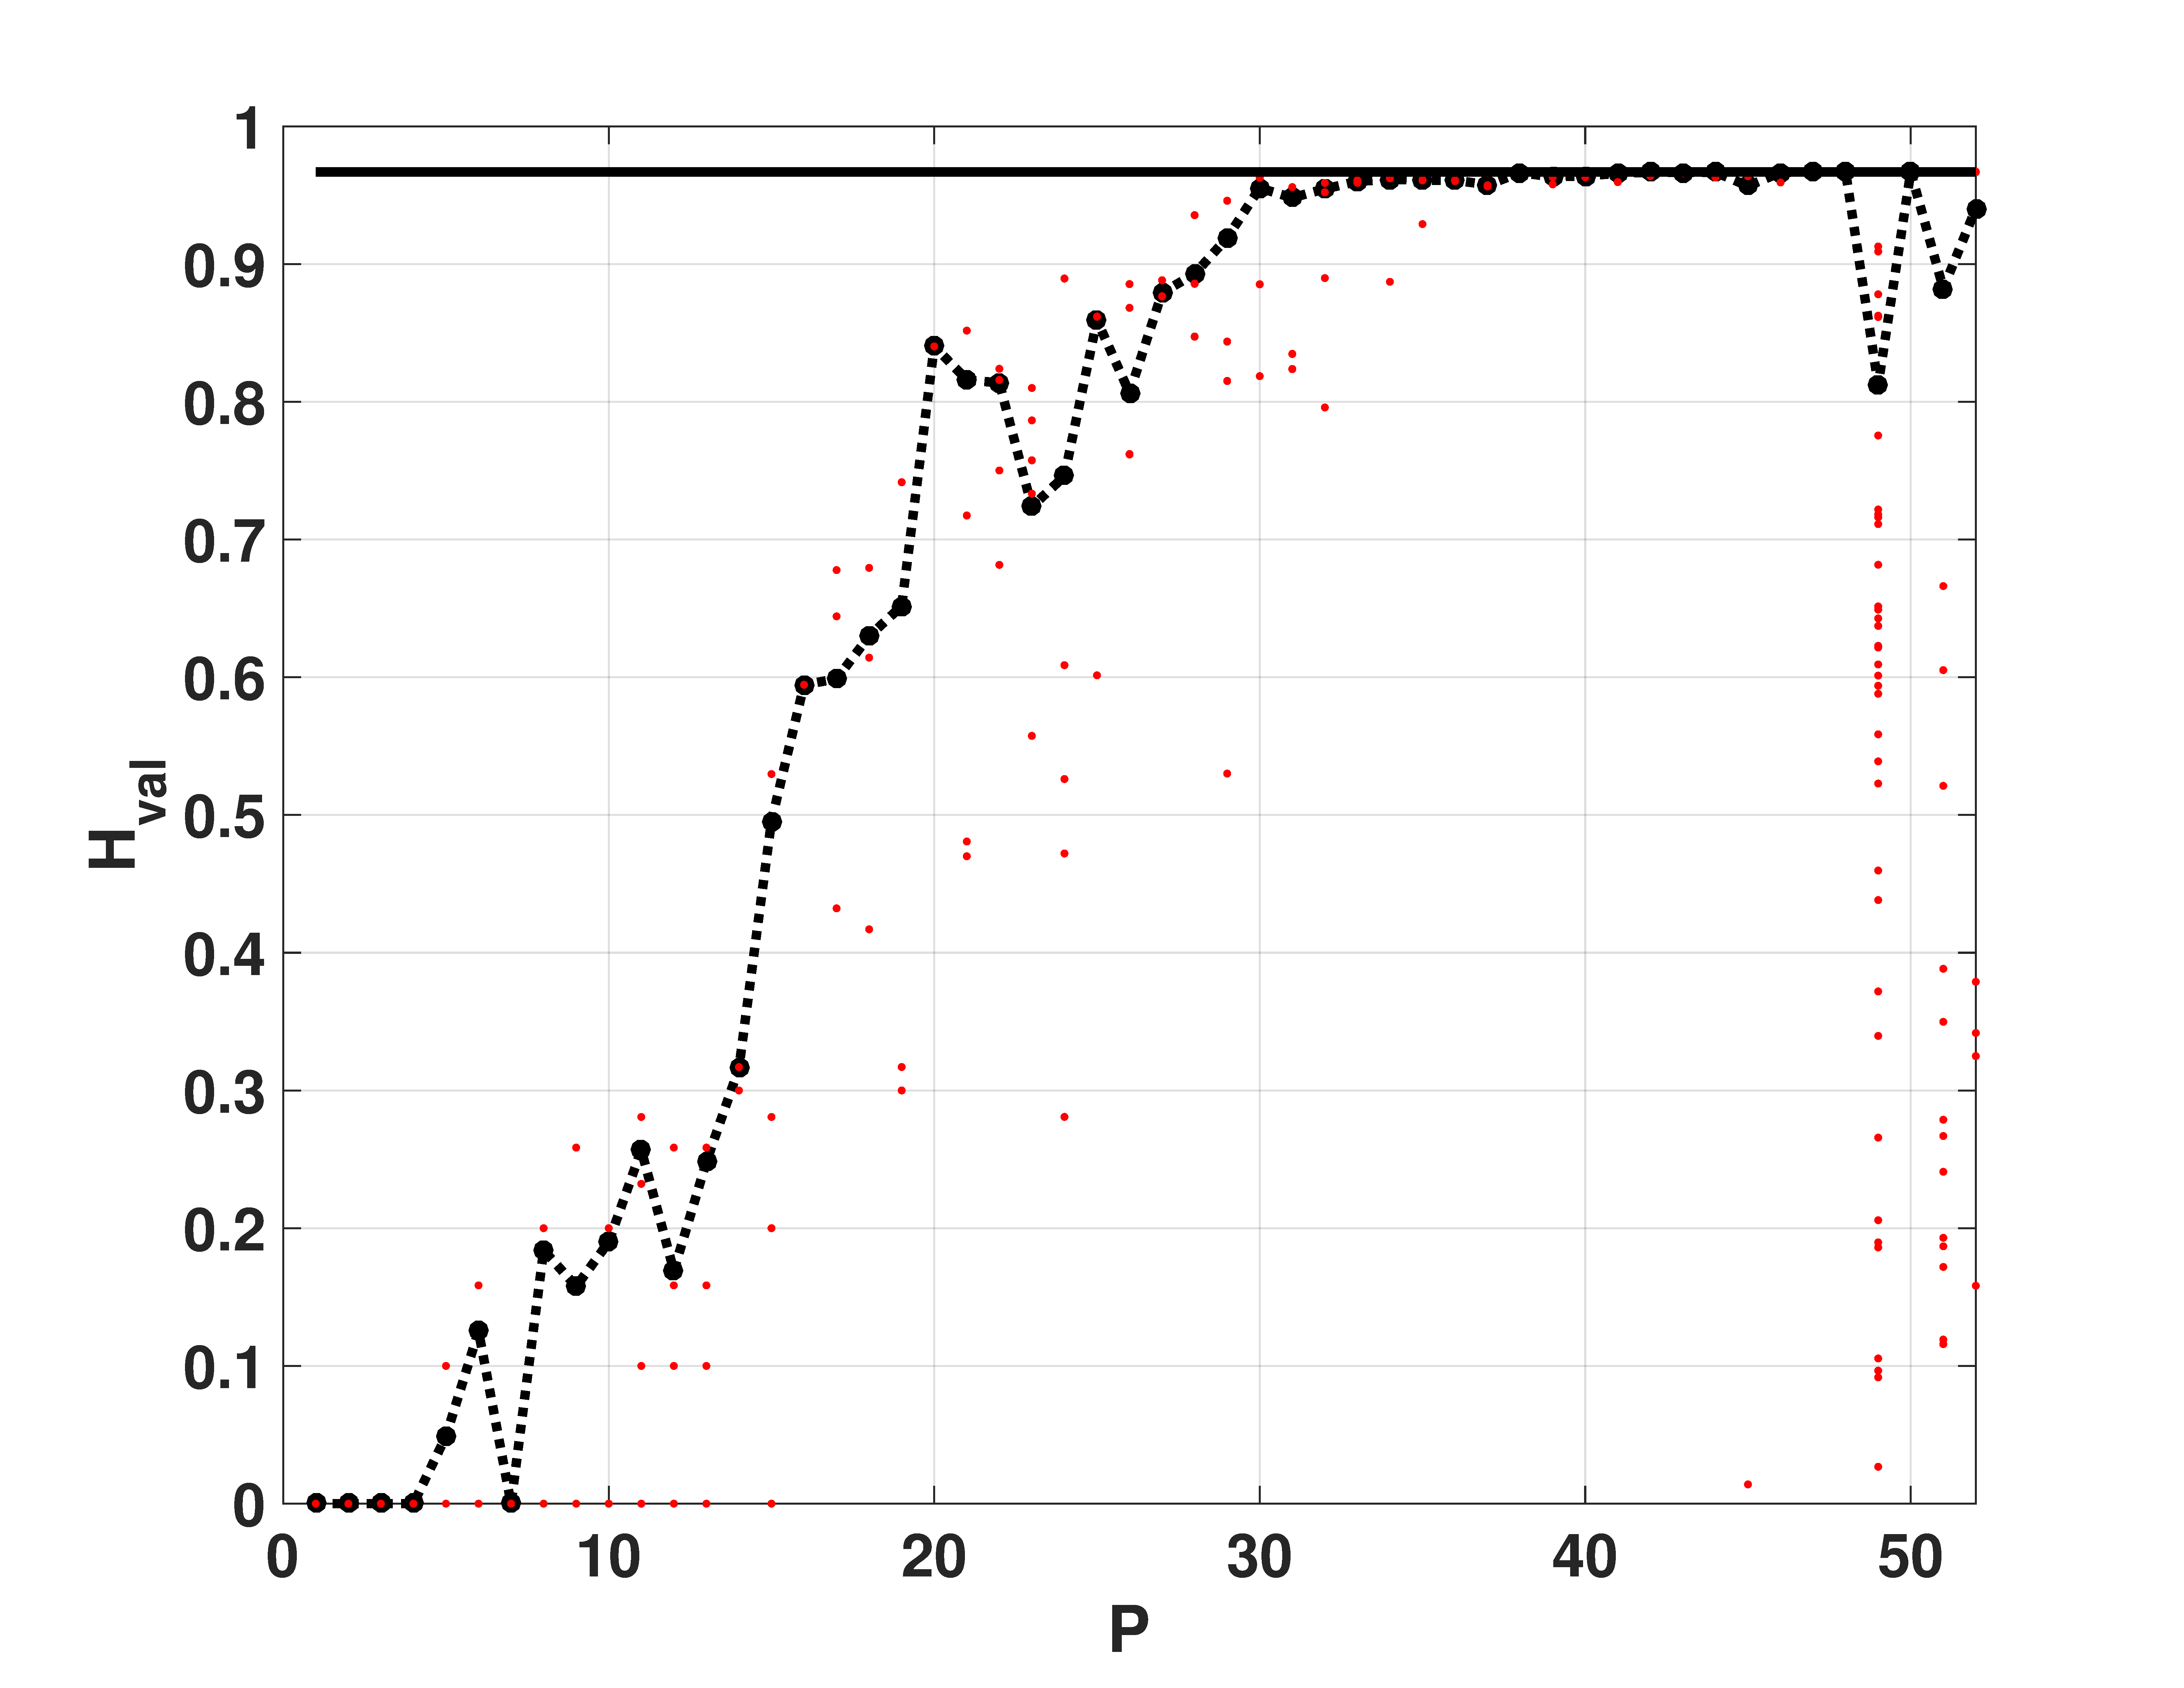
\includegraphics[width=.32\textwidth]{Hval_Logistico}
	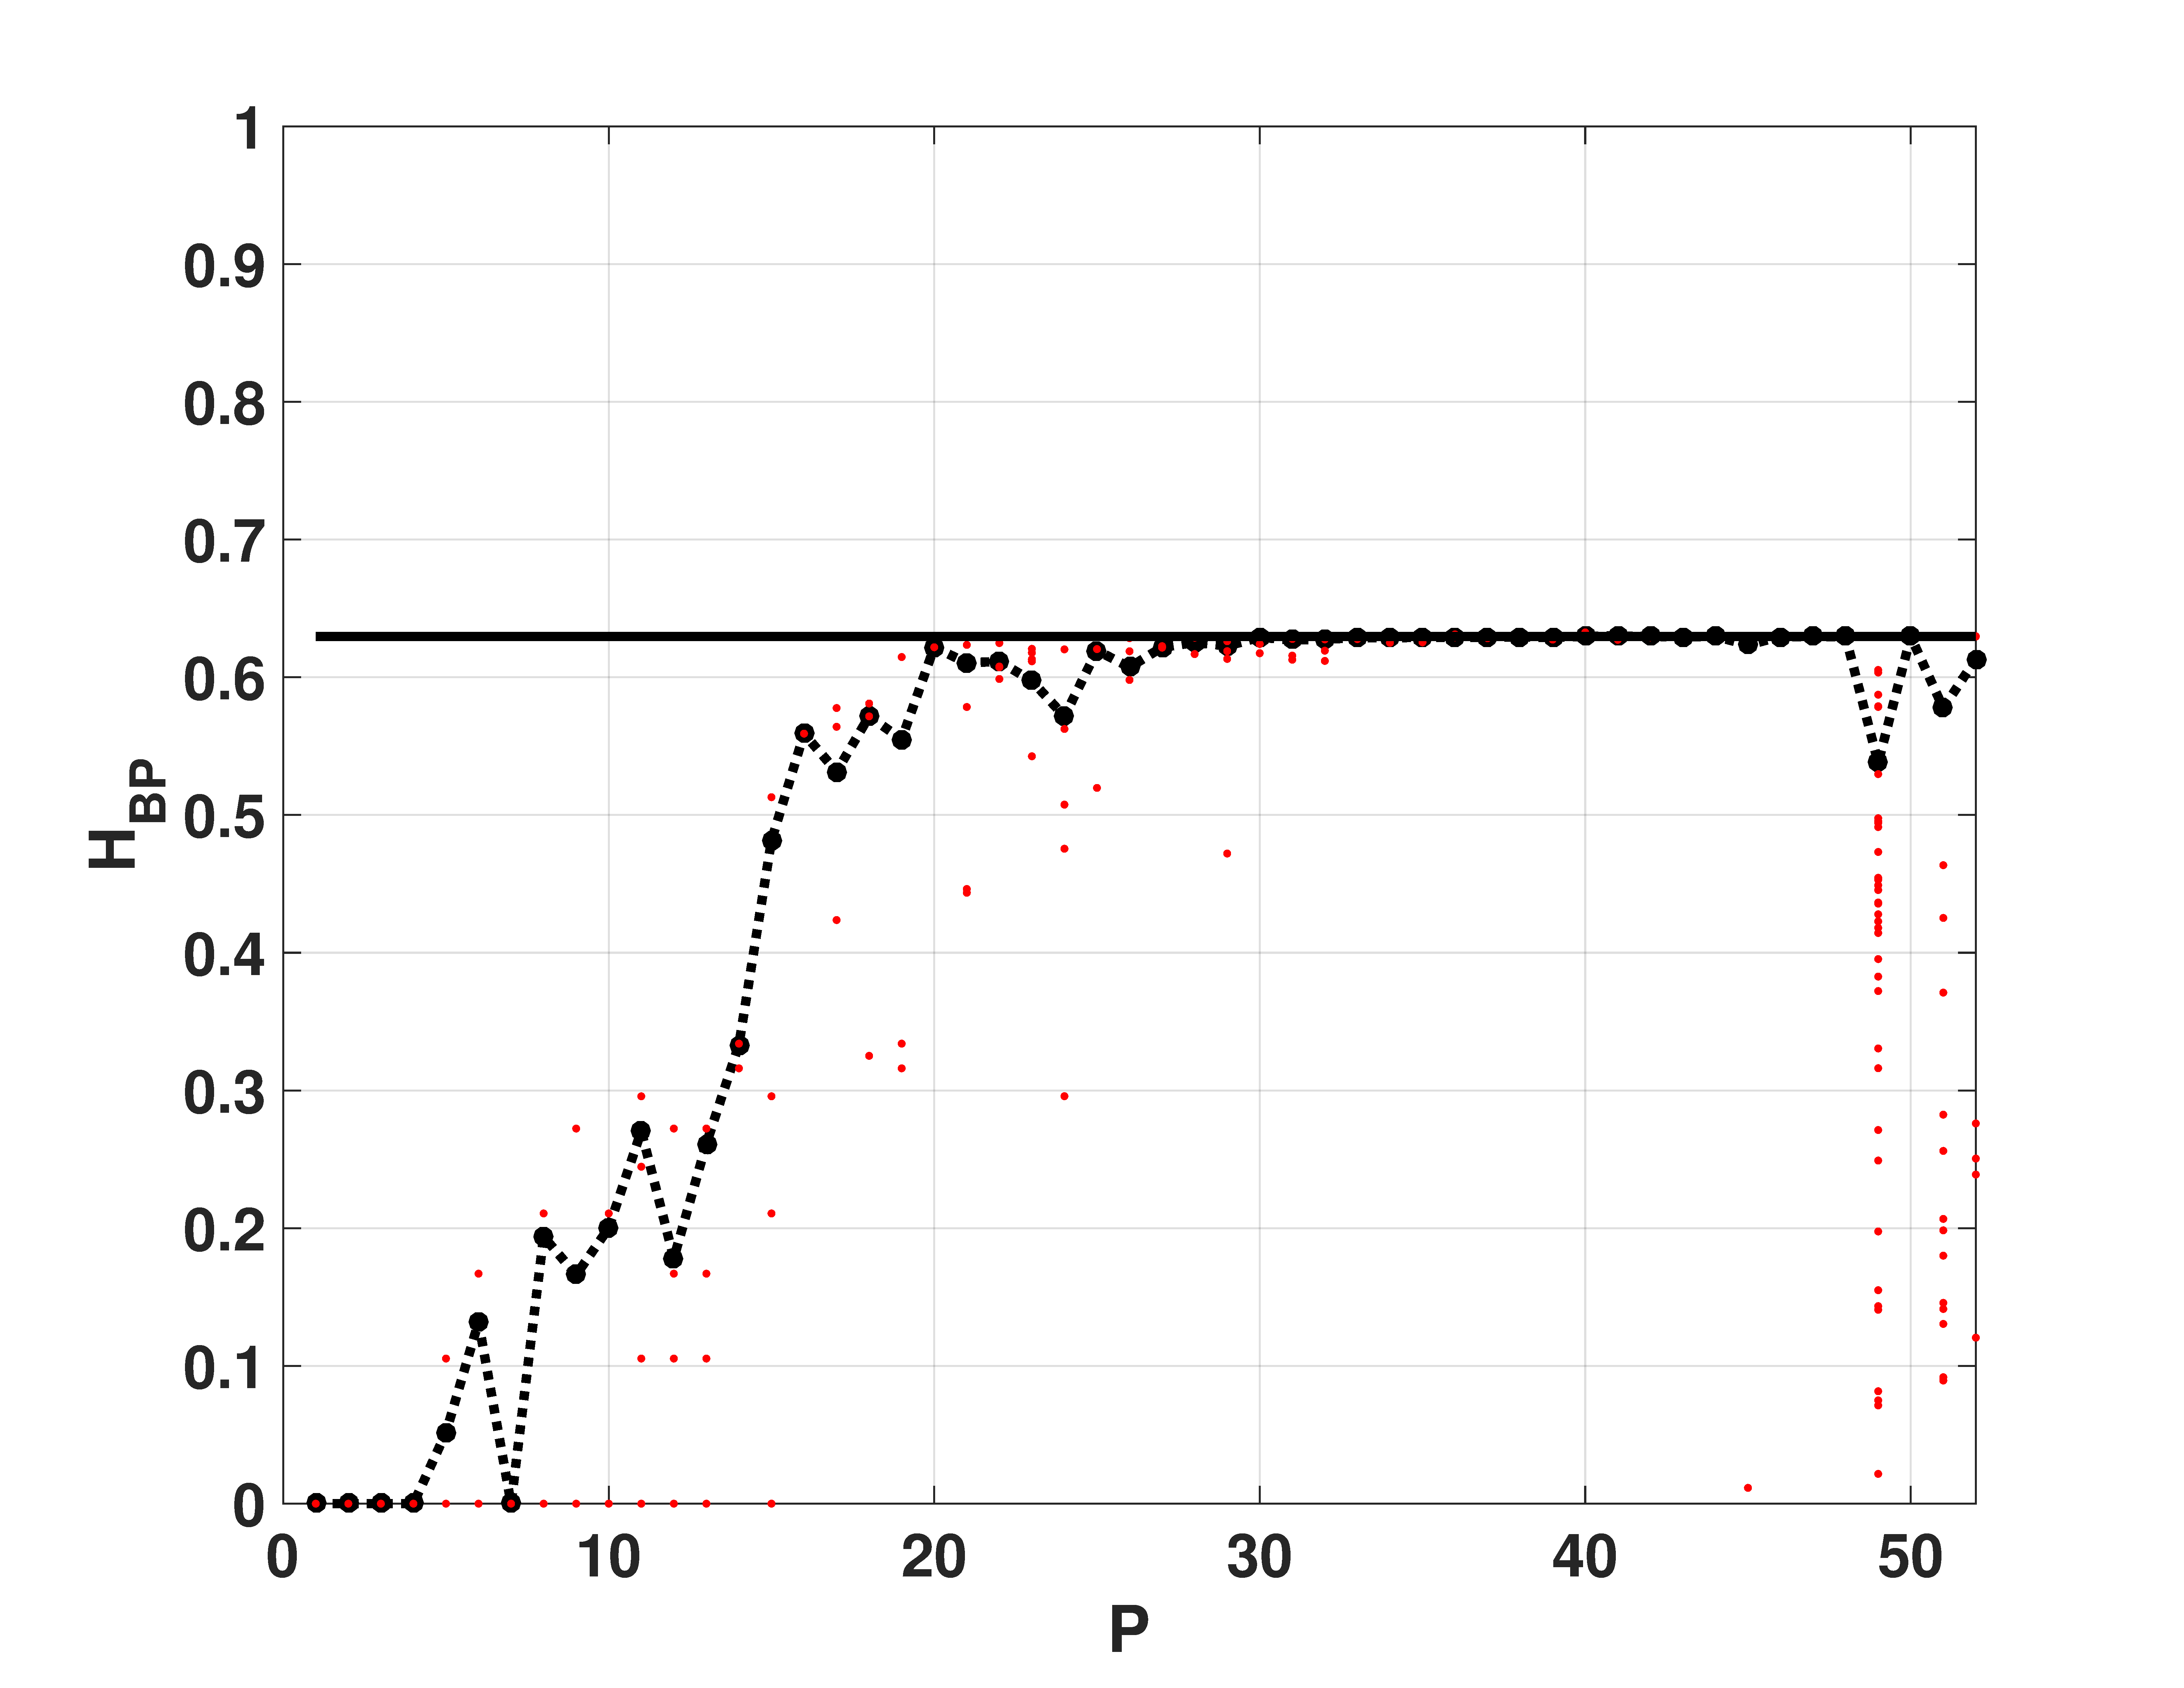
\includegraphics[width=.32\textwidth]{Hbp_Logistico}
	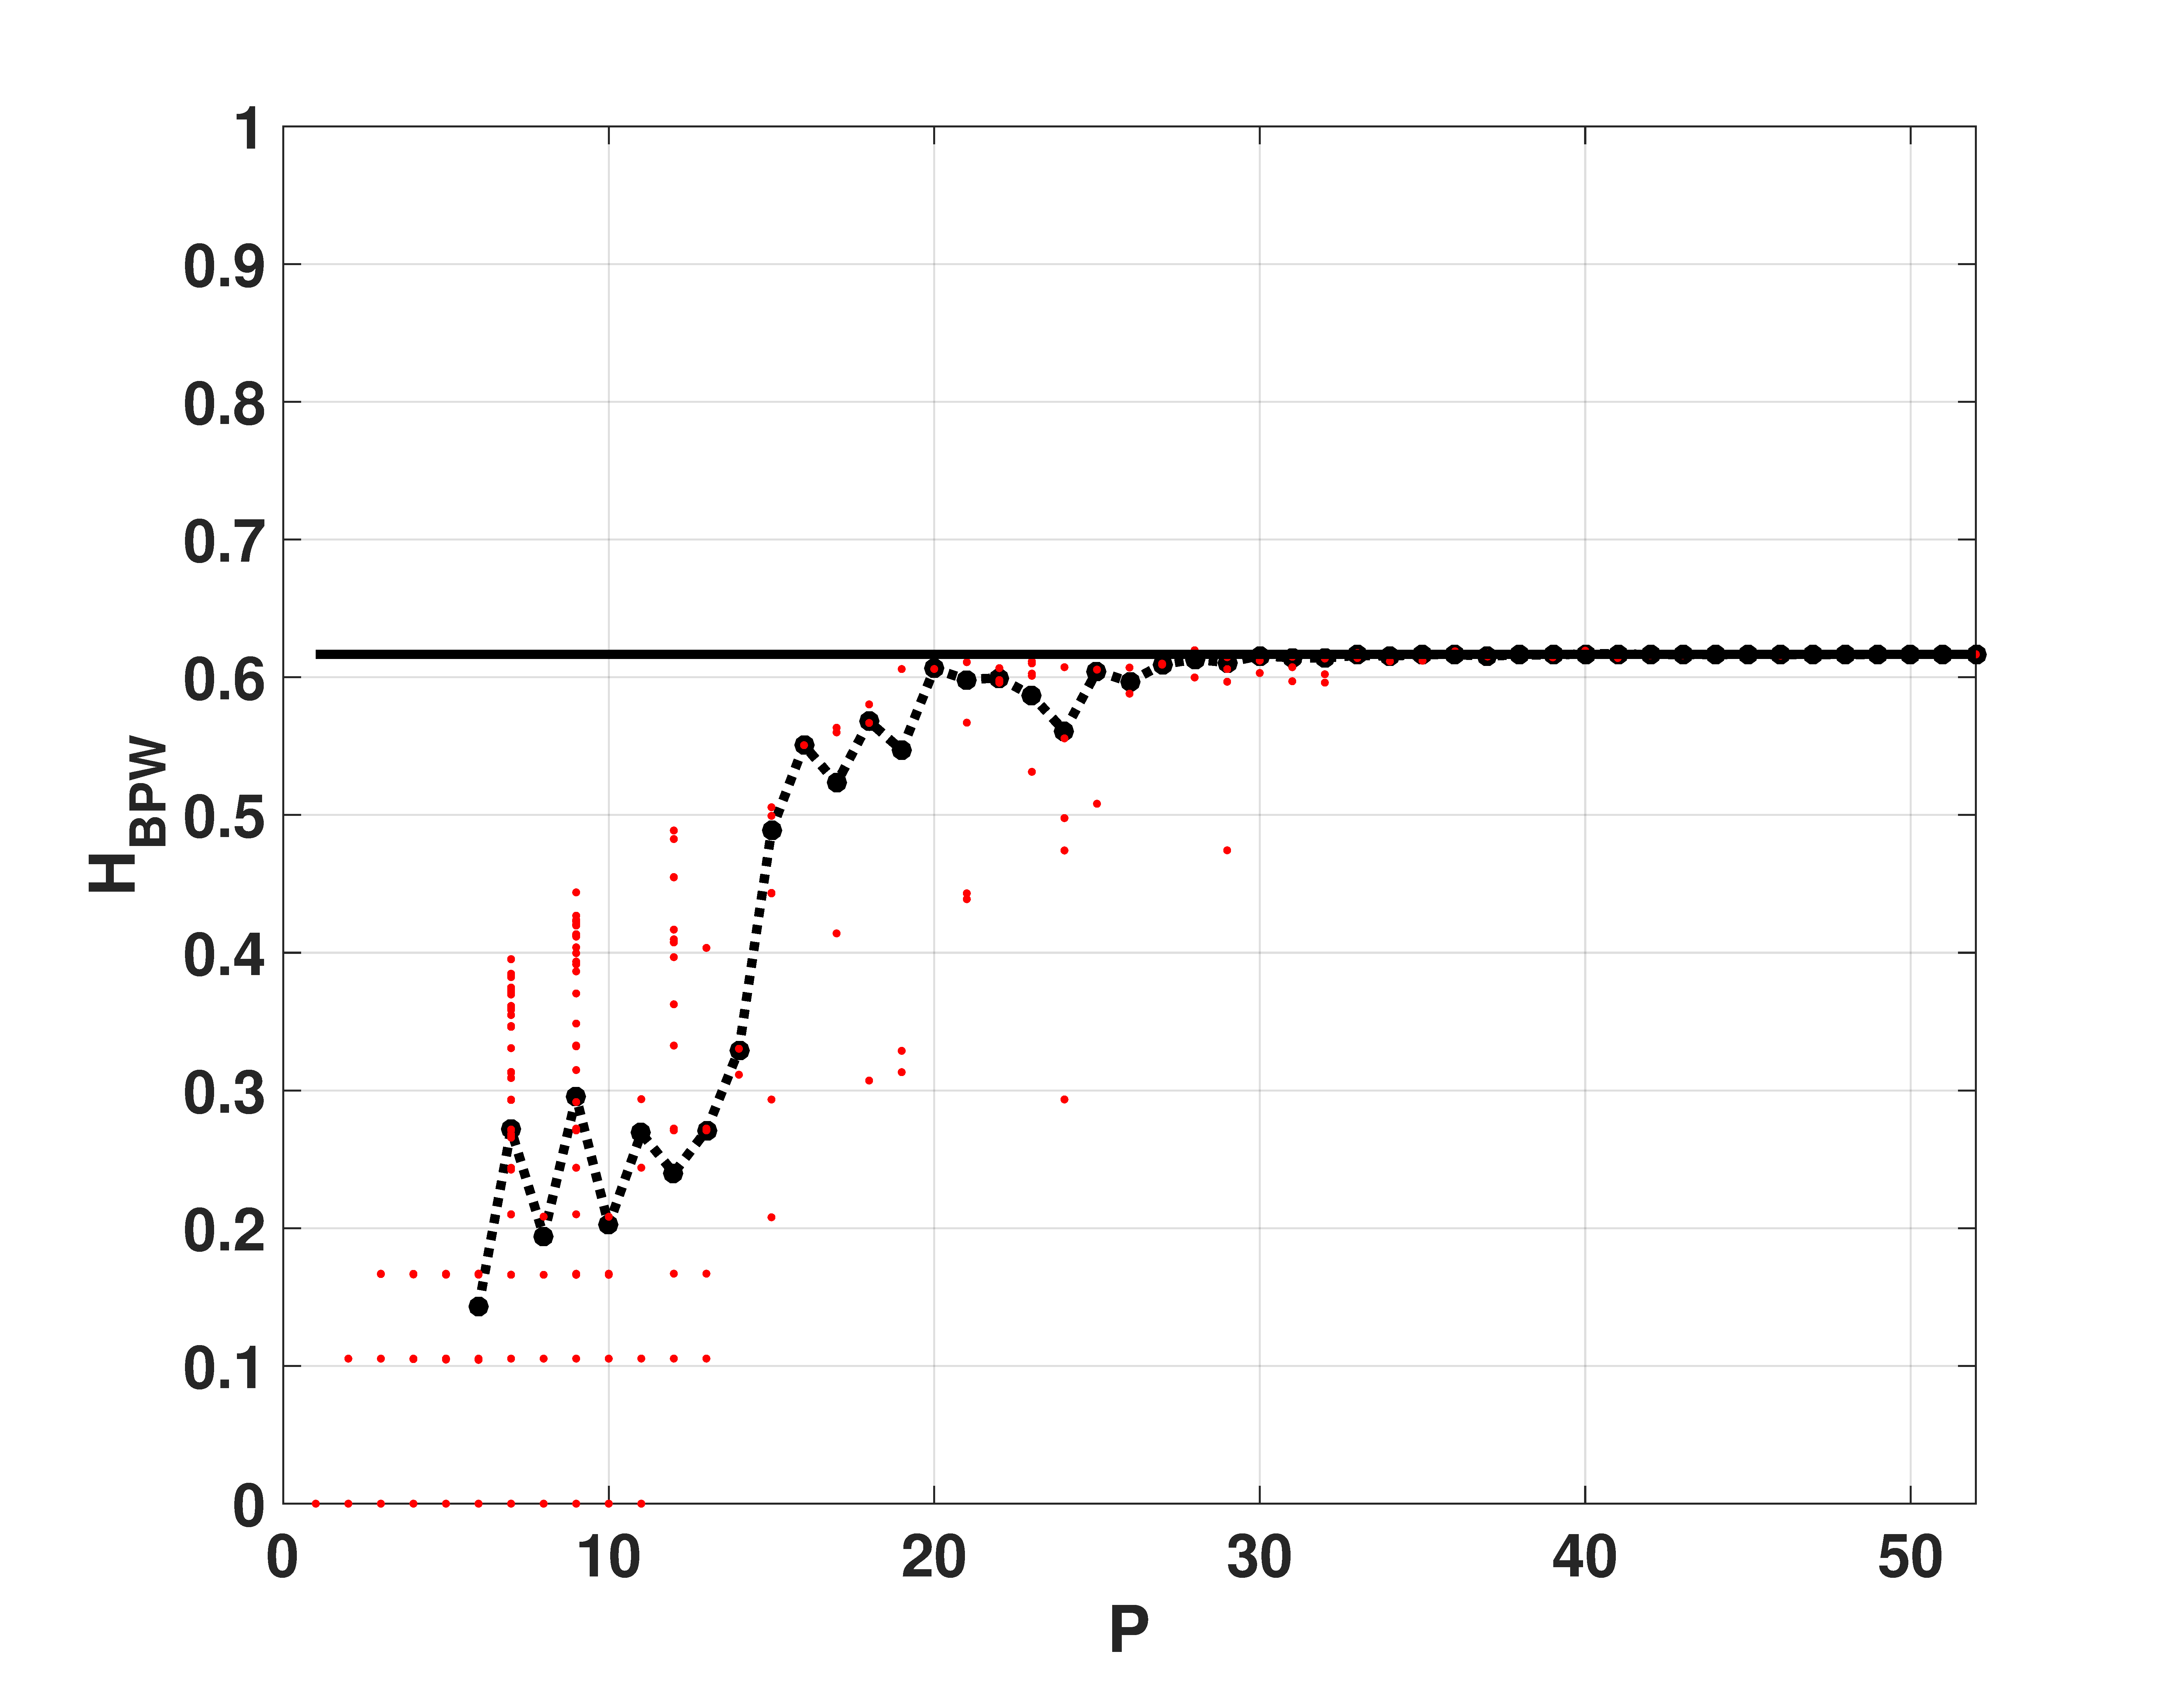
\includegraphics[width=.32\textwidth]{Hbpw_Logistico}
	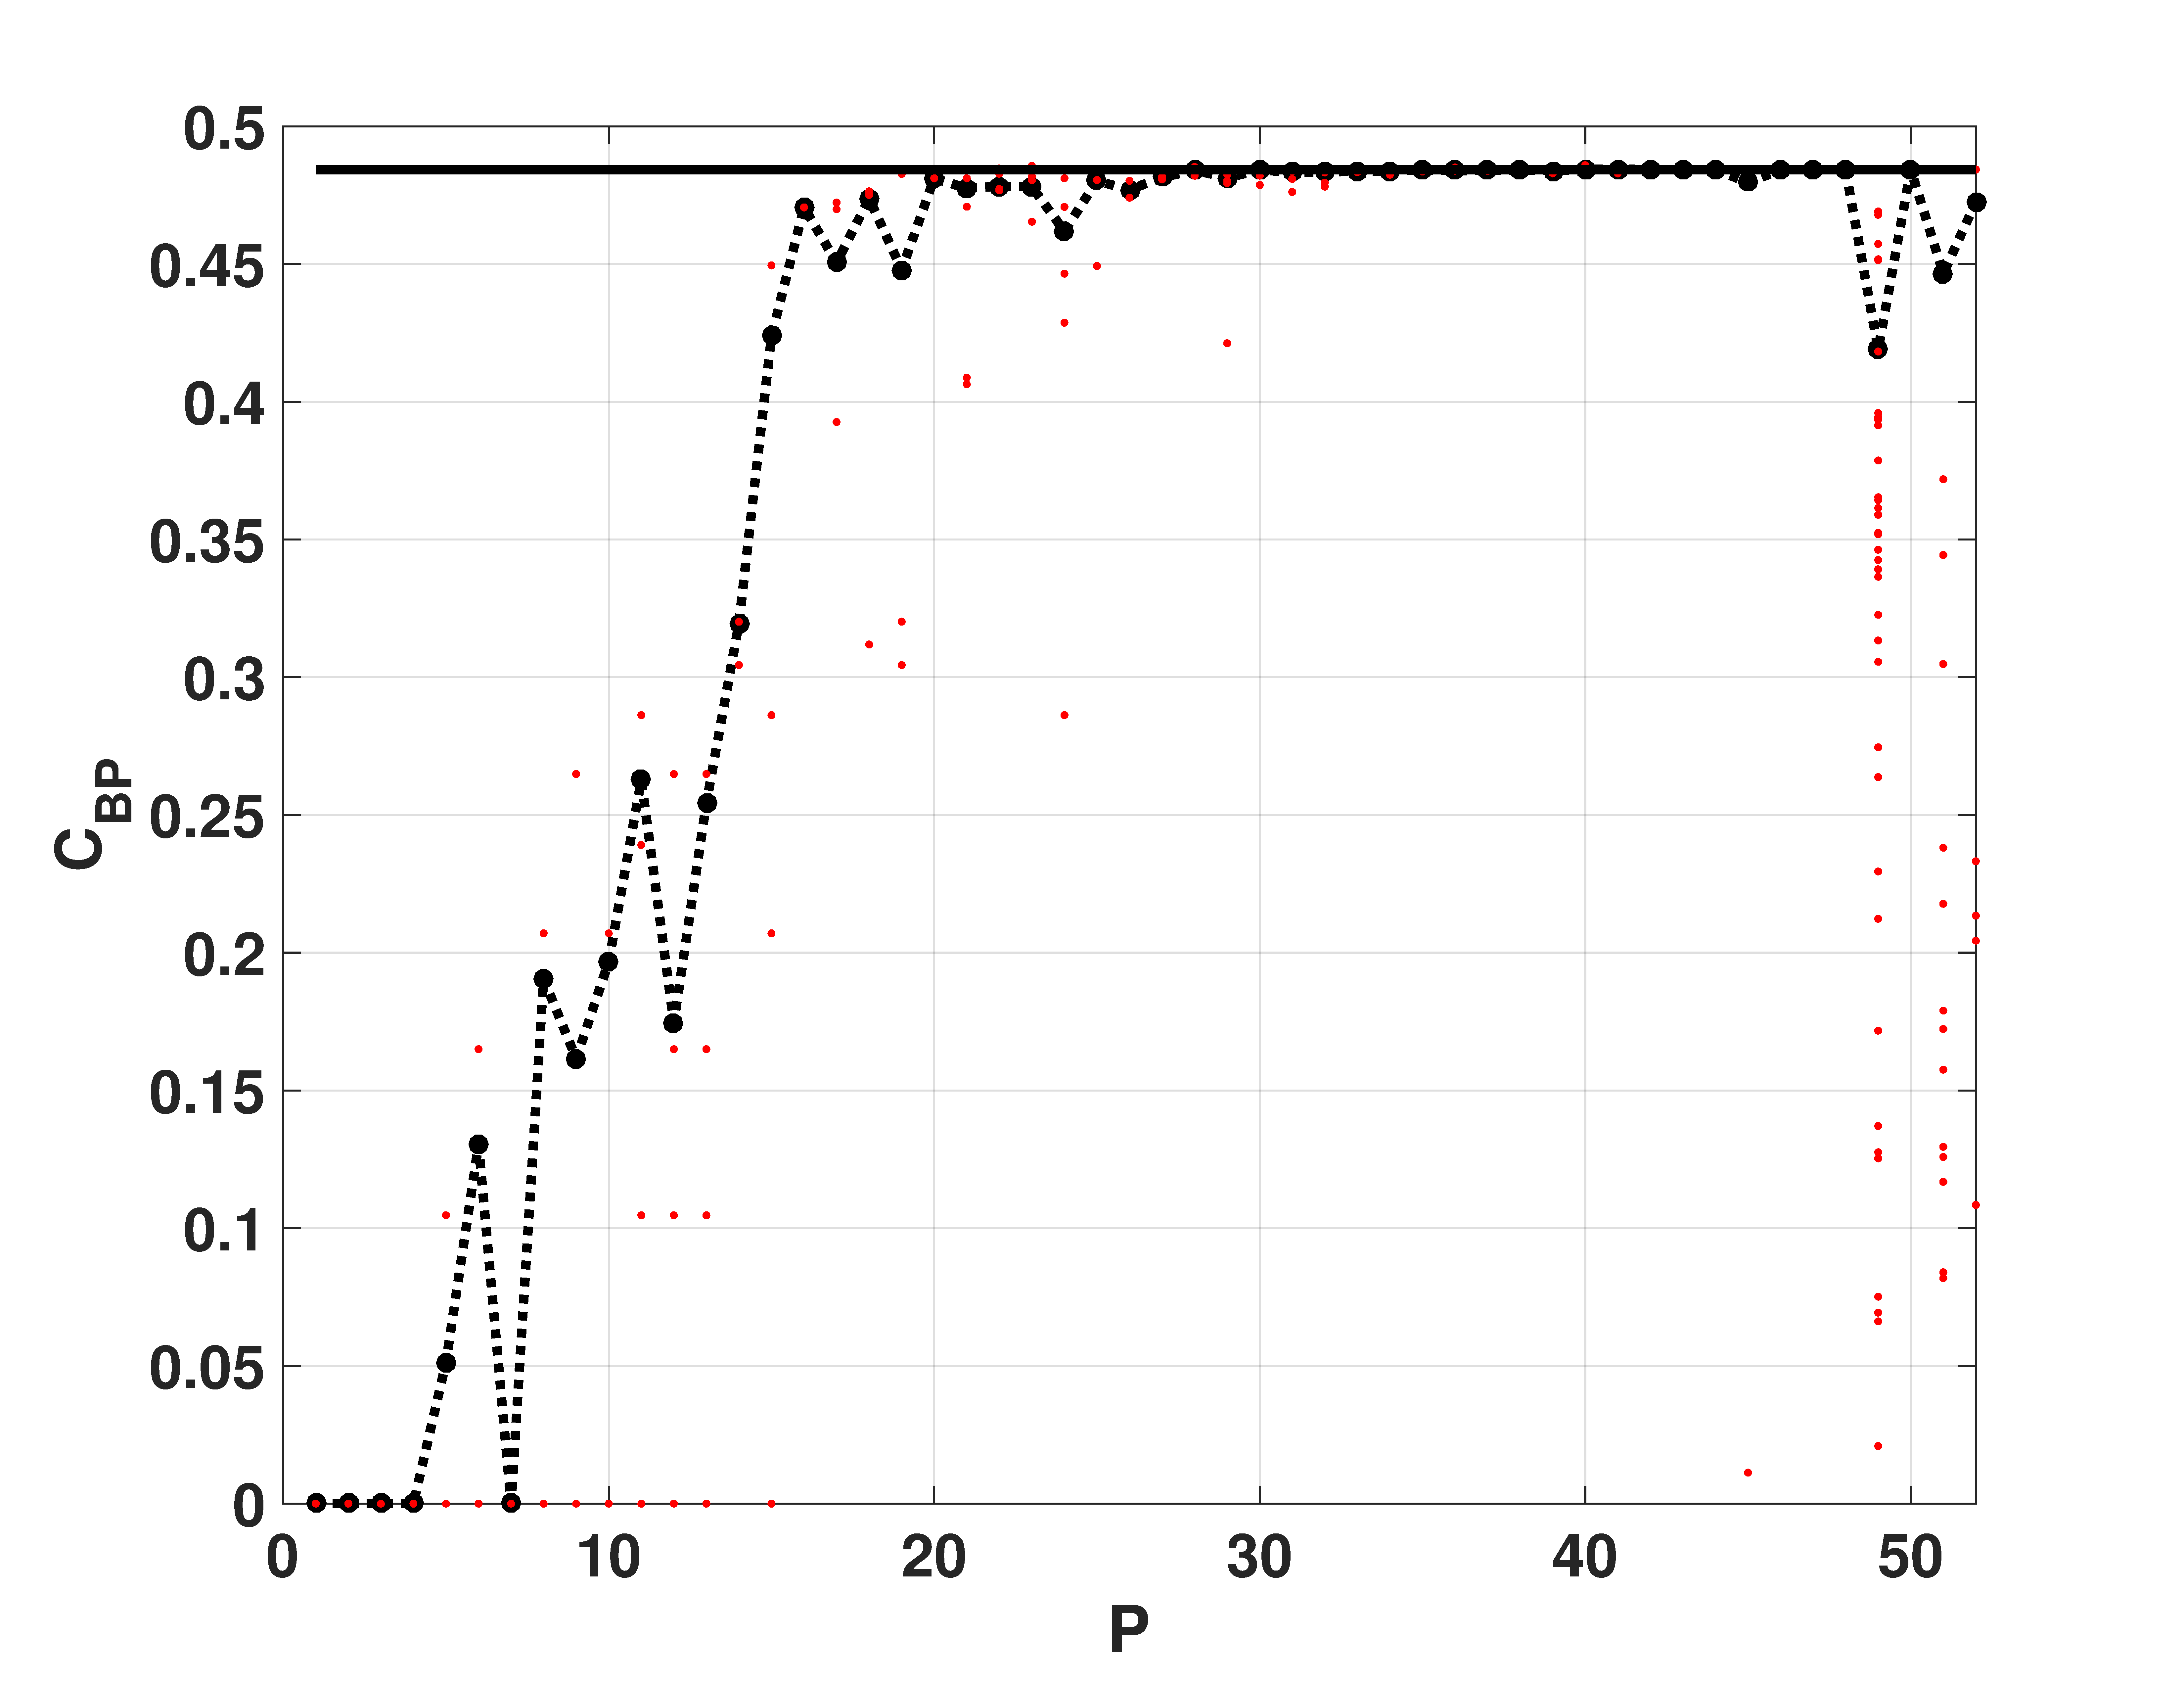
\includegraphics[width=.32\textwidth]{Cbp_Logistico}
	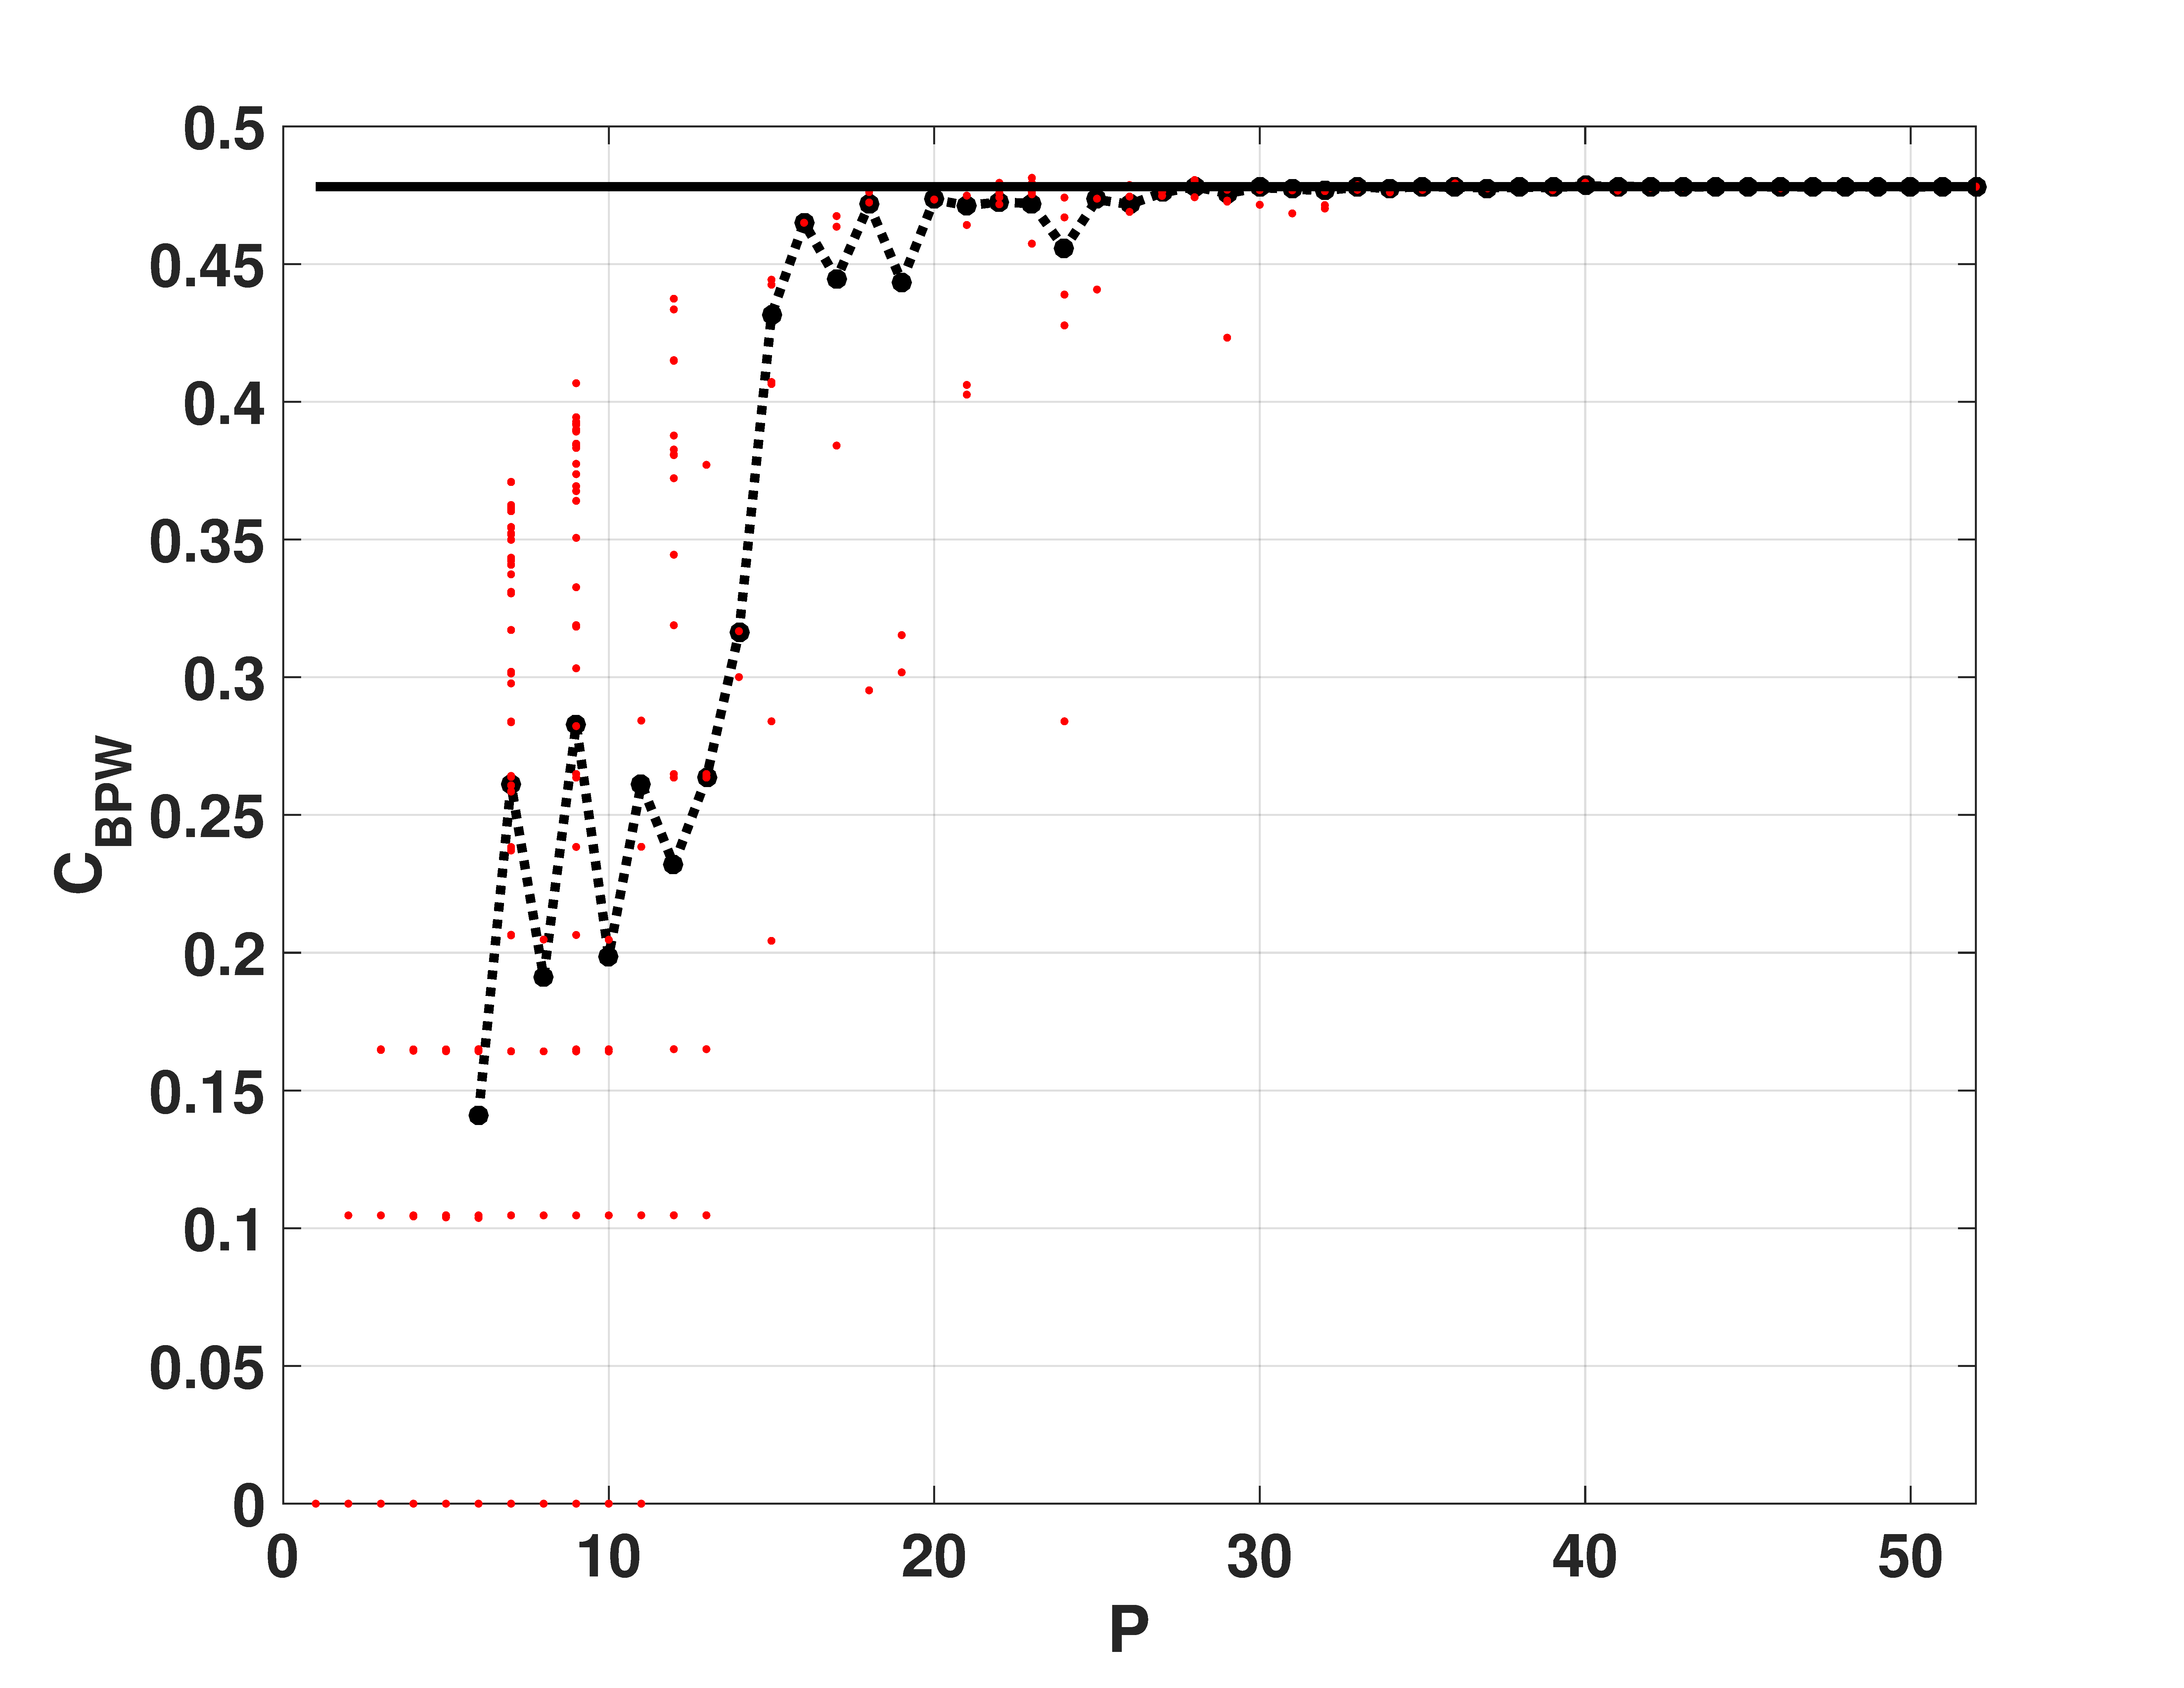
\includegraphics[width=.32\textwidth]{Cbpw_Logistico}
	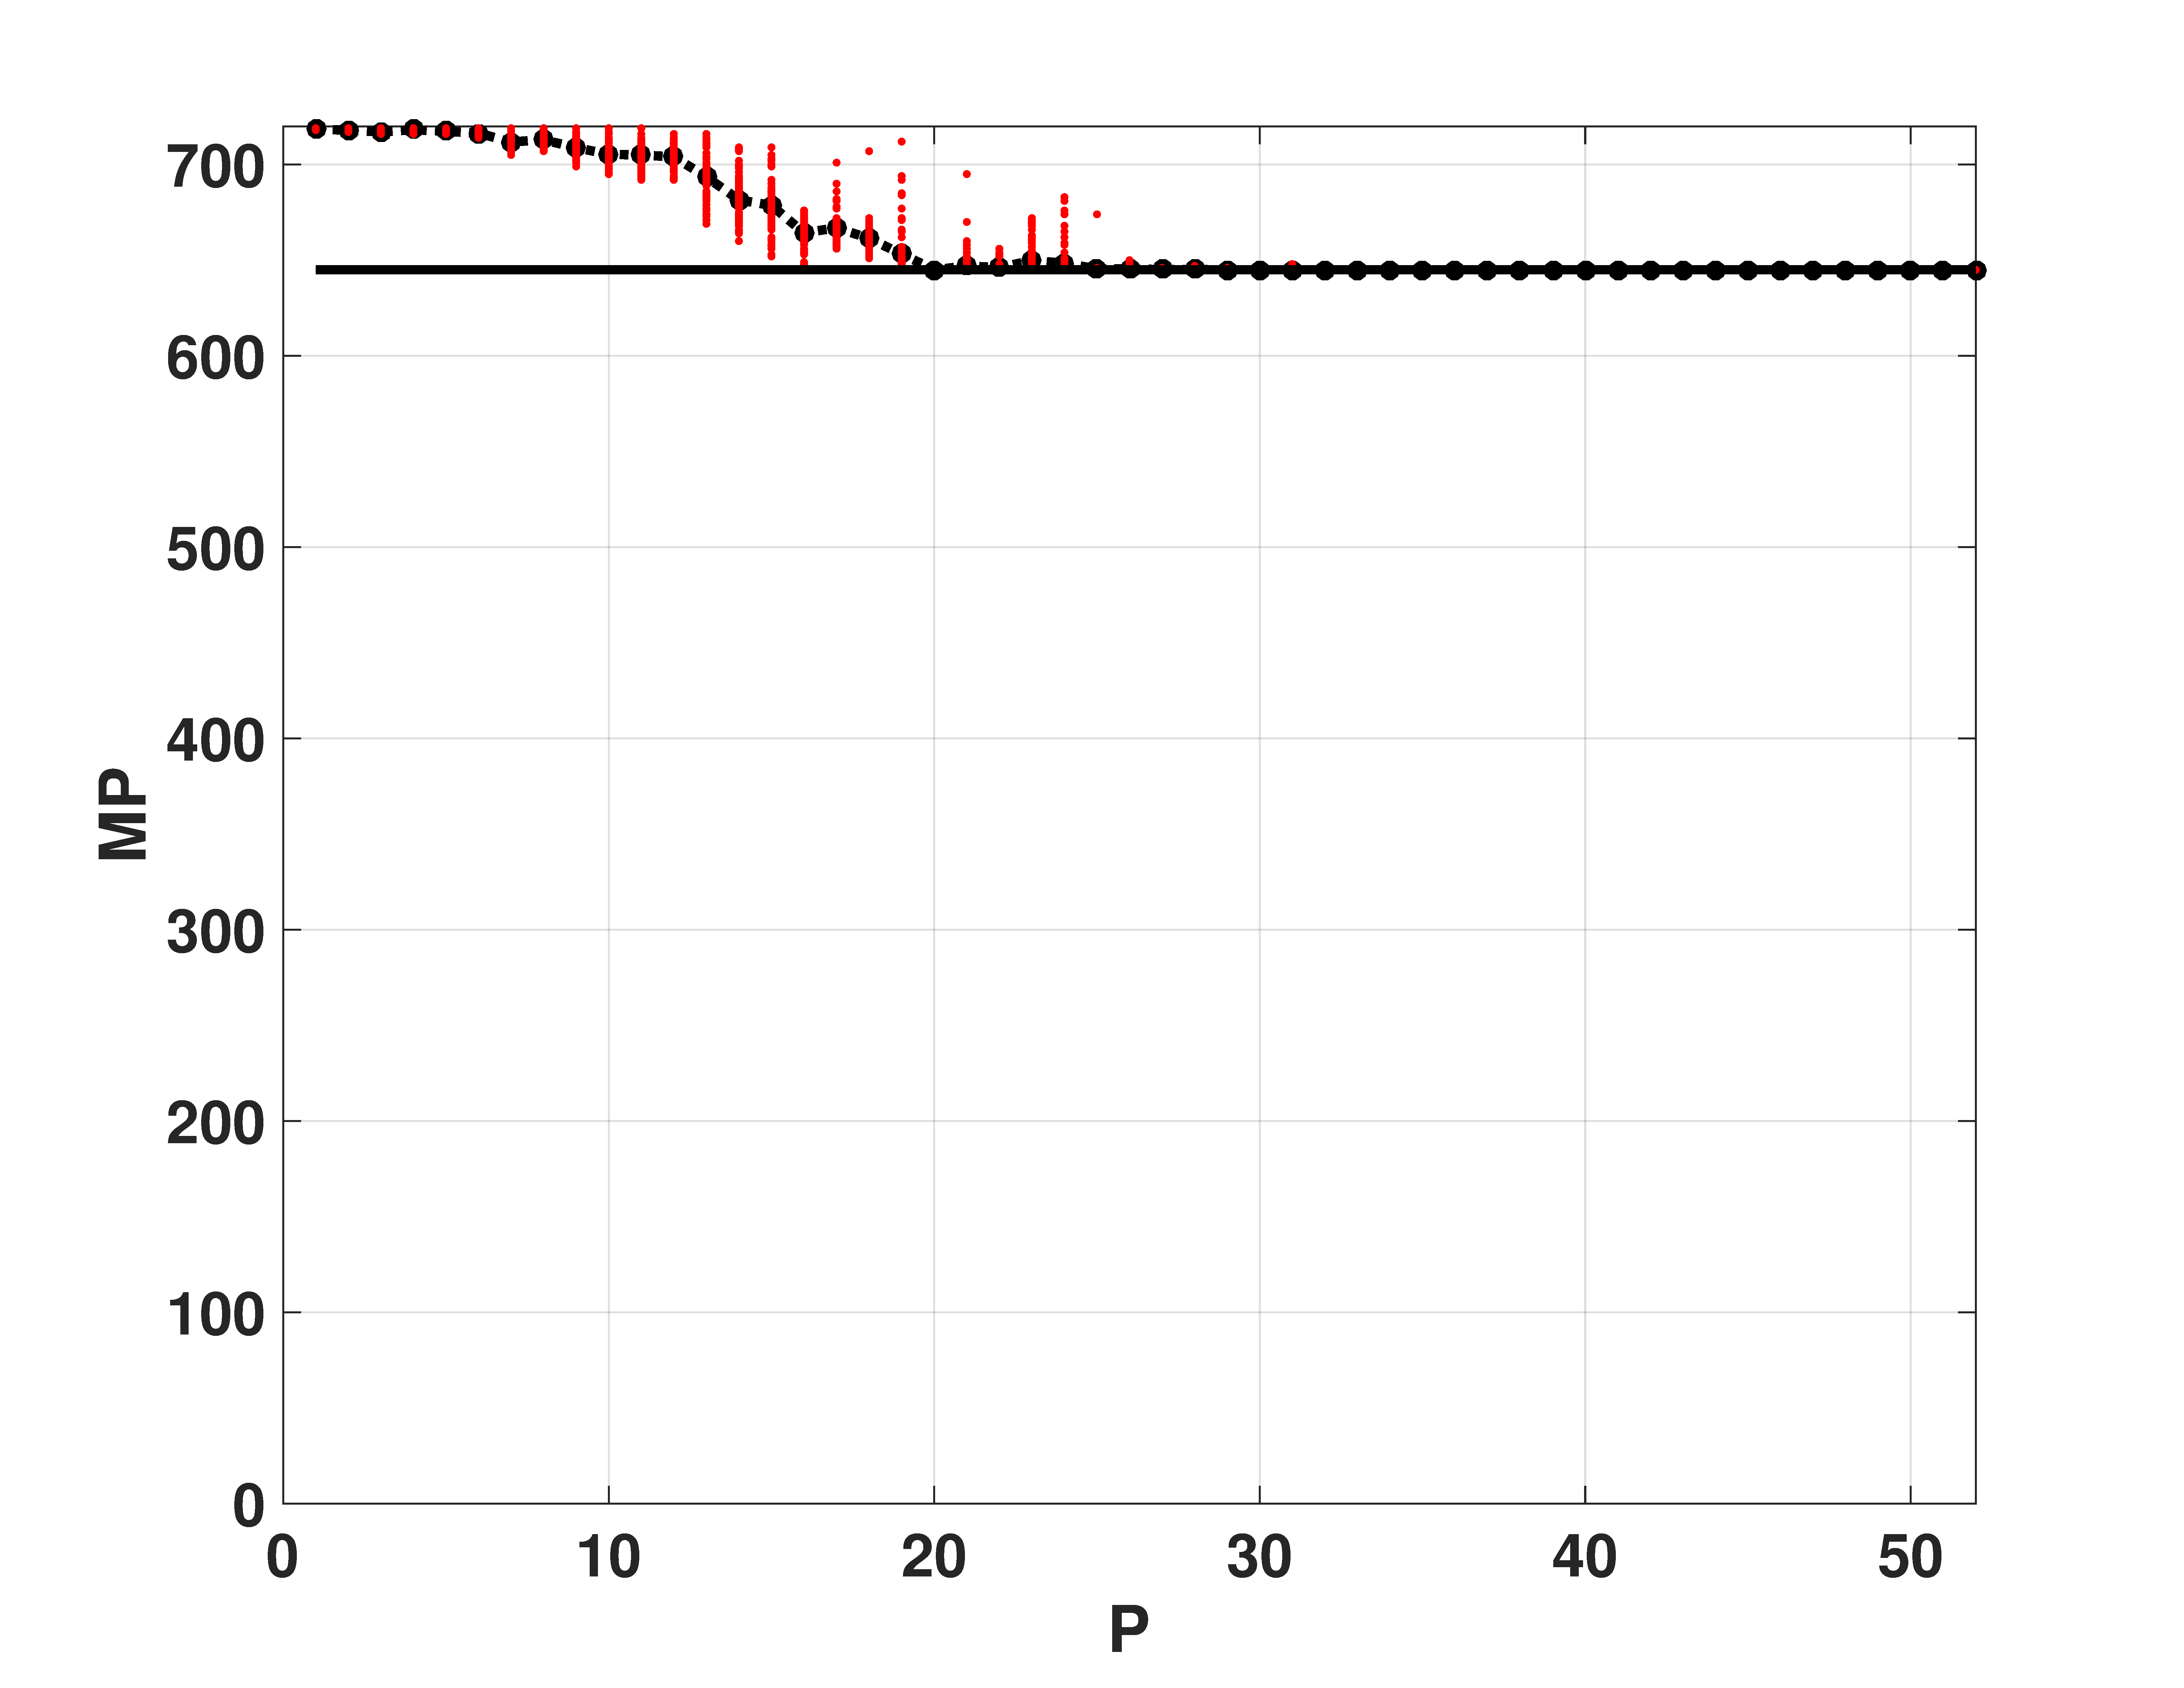
\includegraphics[width=.32\textwidth]{MP_Logistico}
	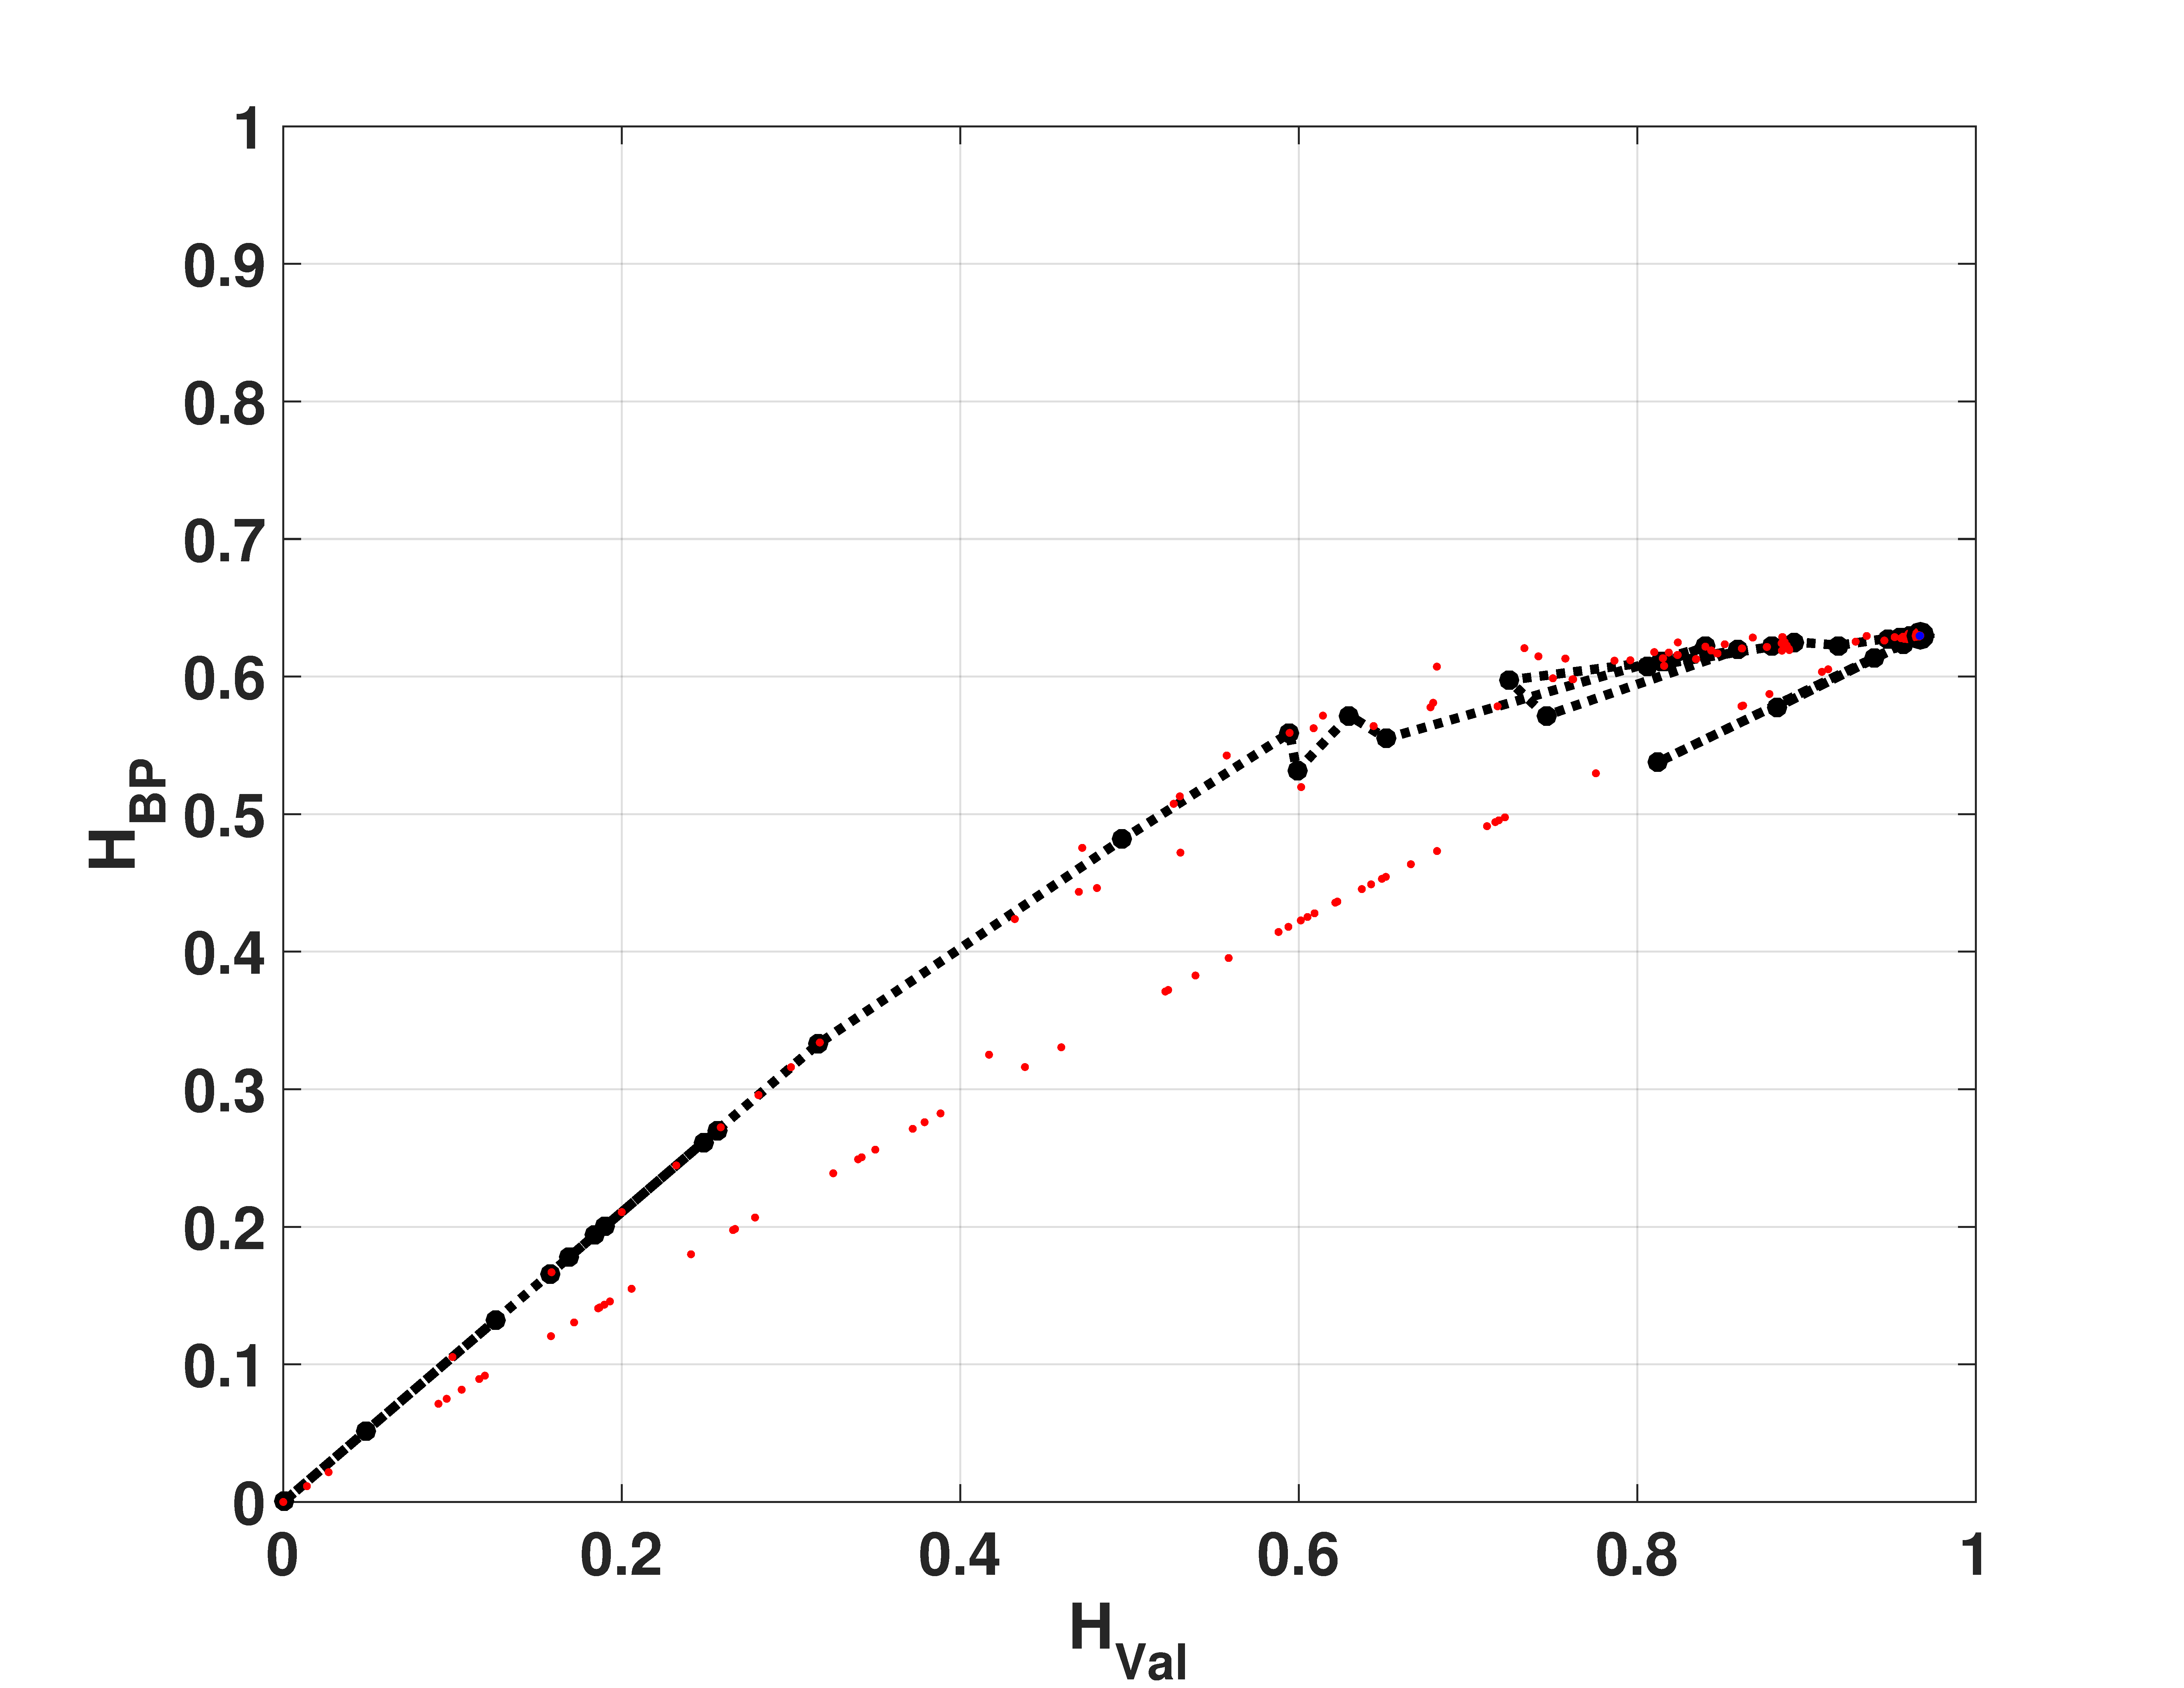
\includegraphics[width=.32\textwidth]{HbpHval_Logistico}
	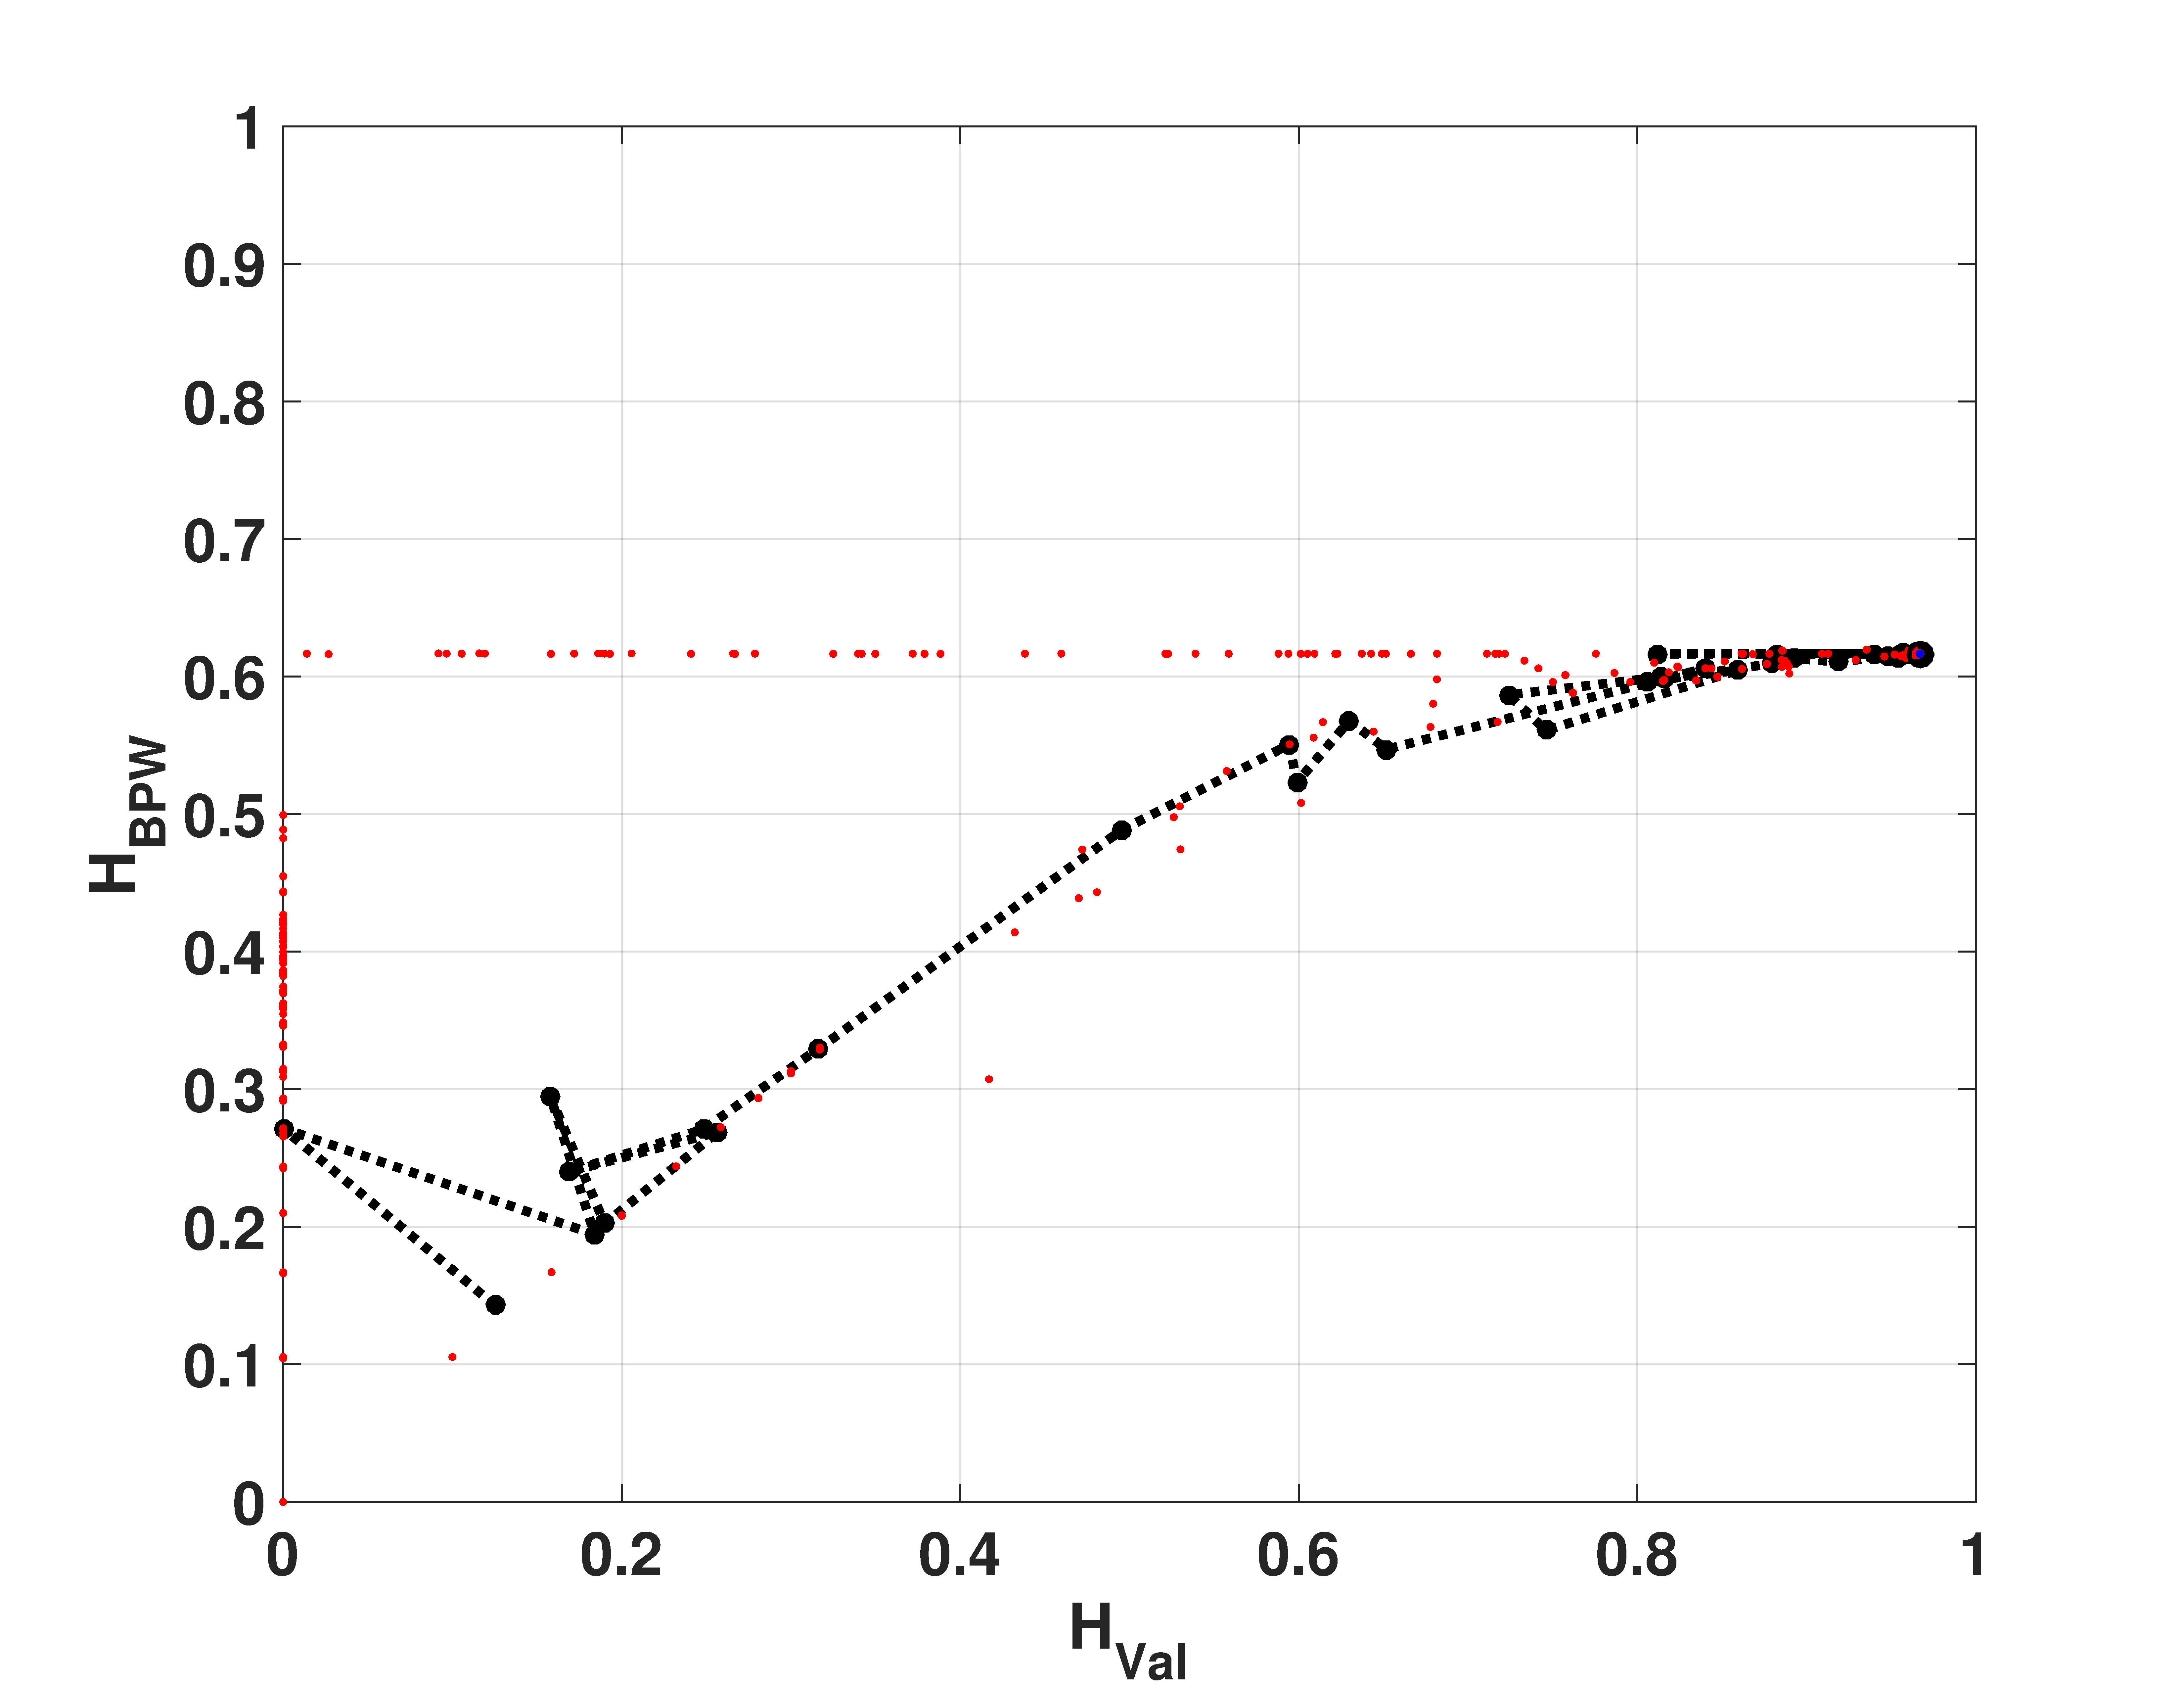
\includegraphics[width=.32\textwidth]{HbpwHval_Logistico}
	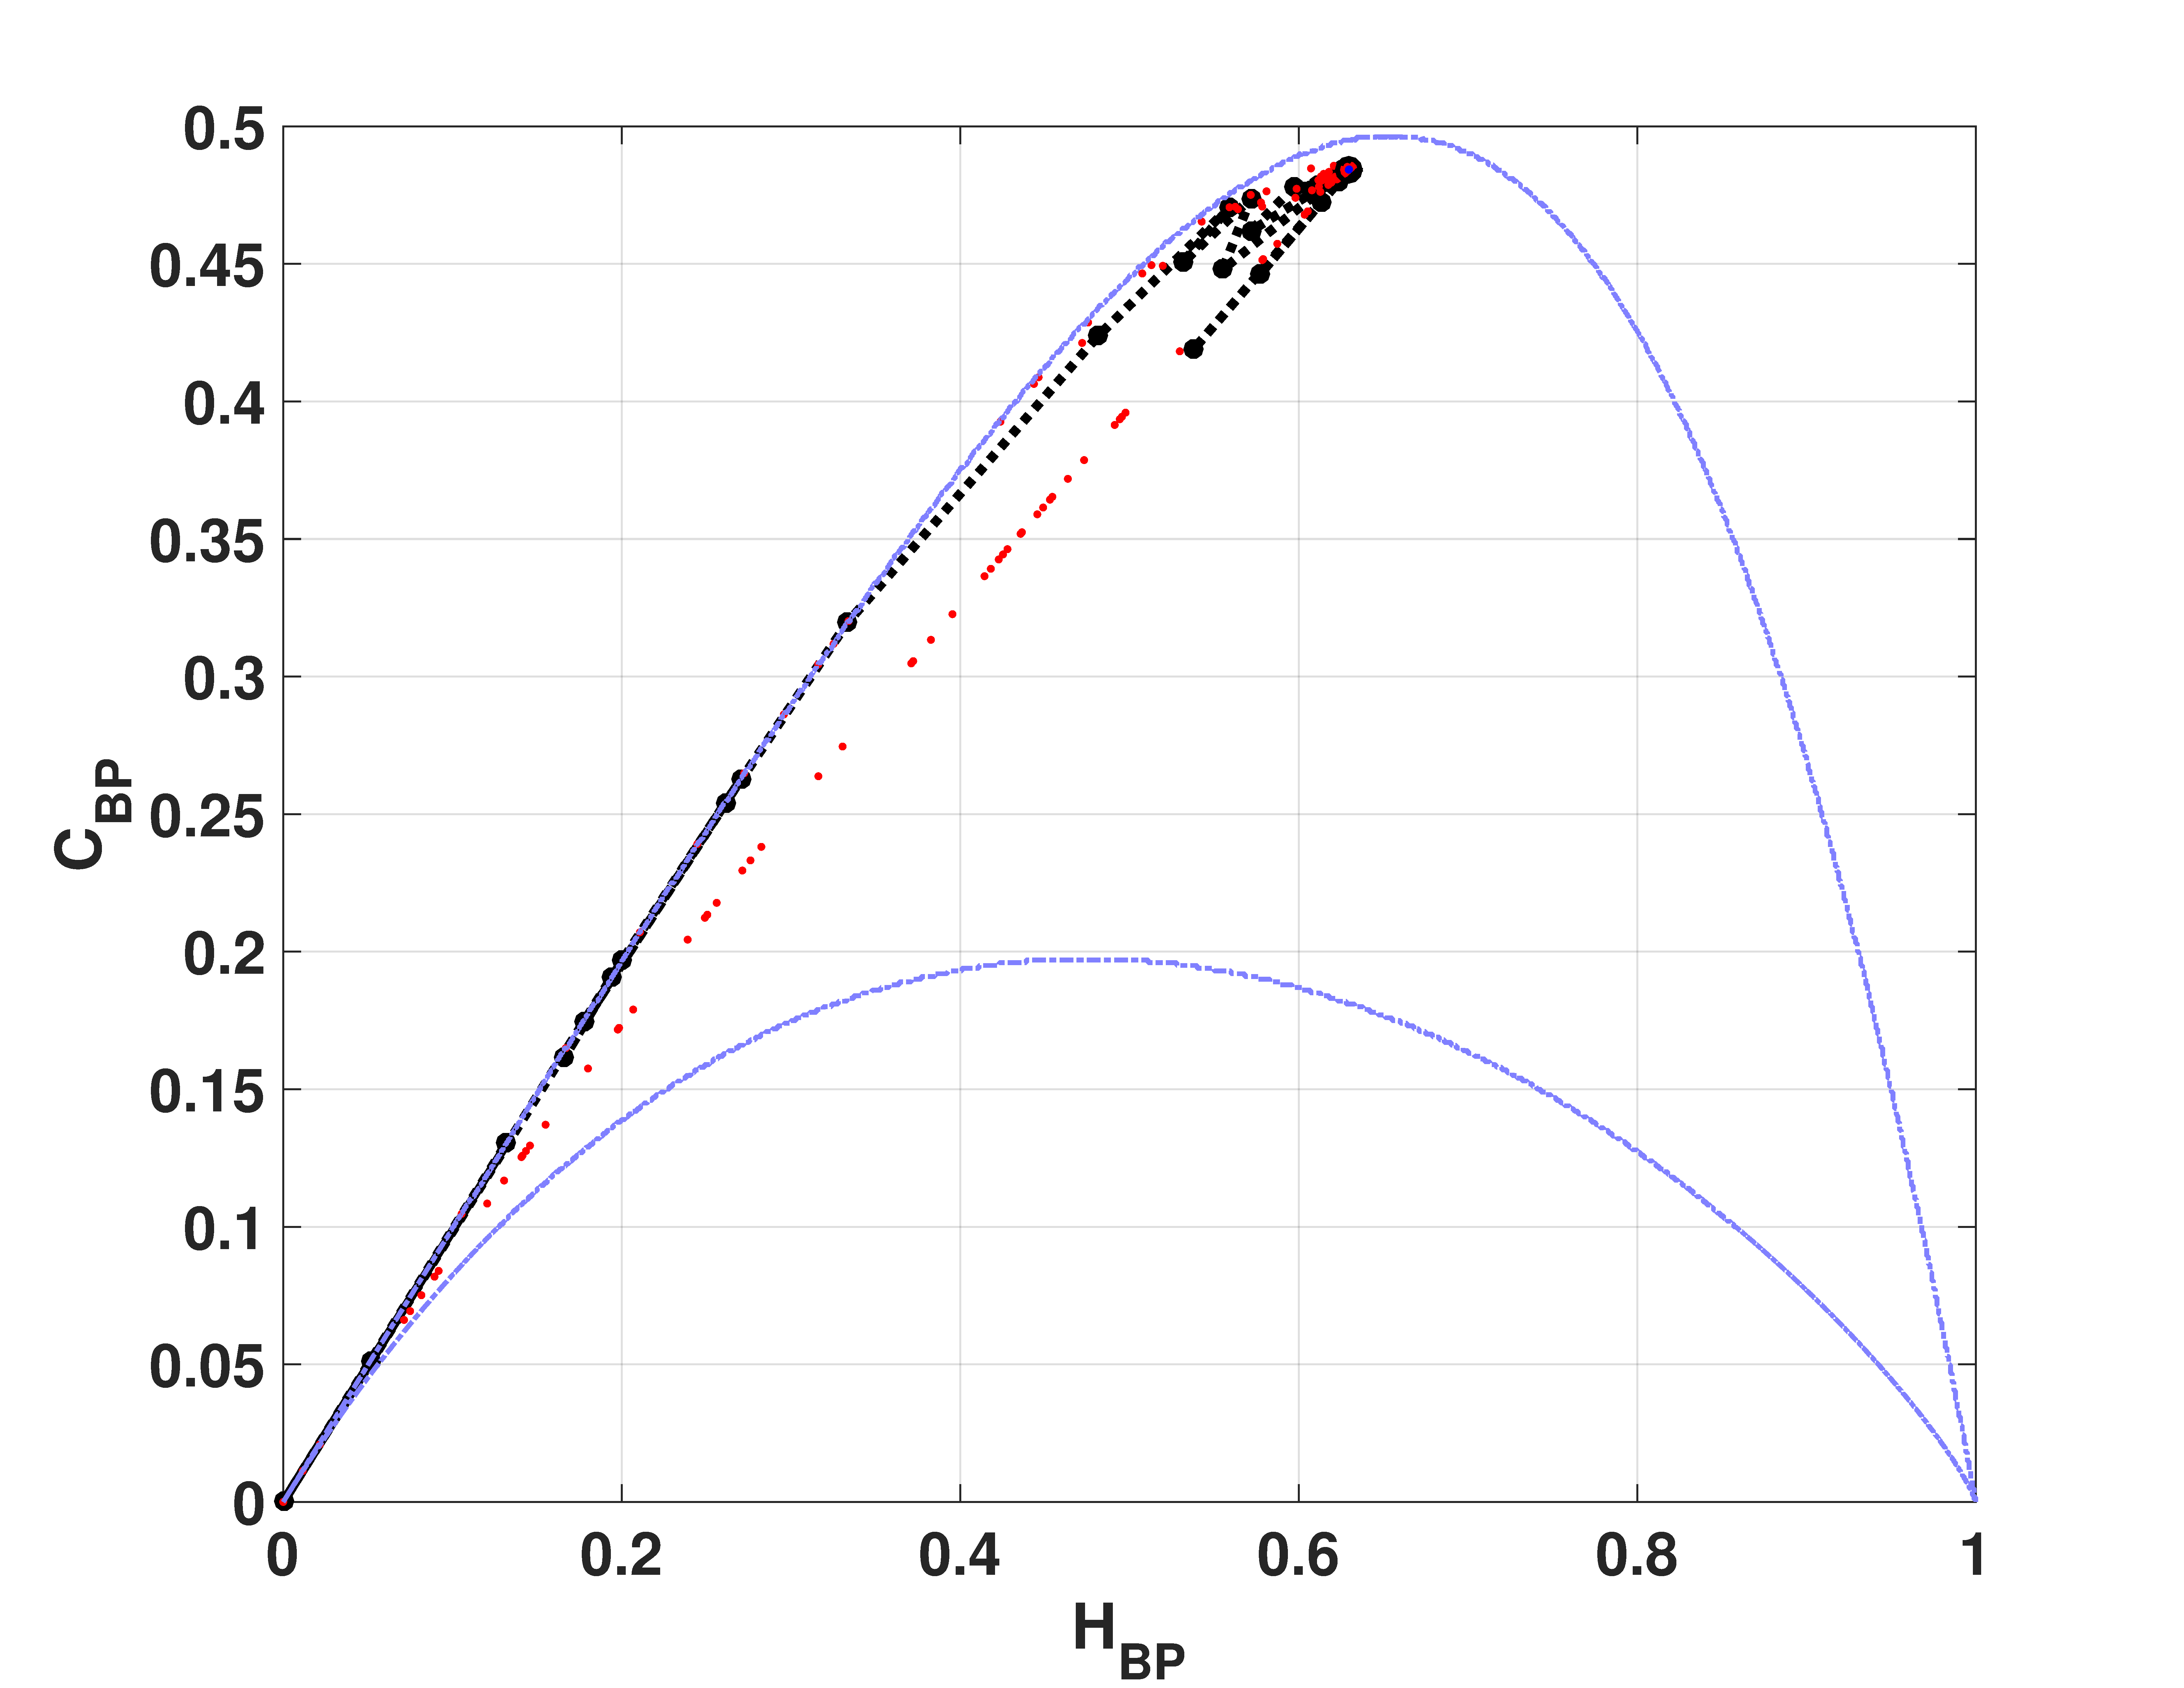
\includegraphics[width=.32\textwidth]{CbpHbp_Logistico}
	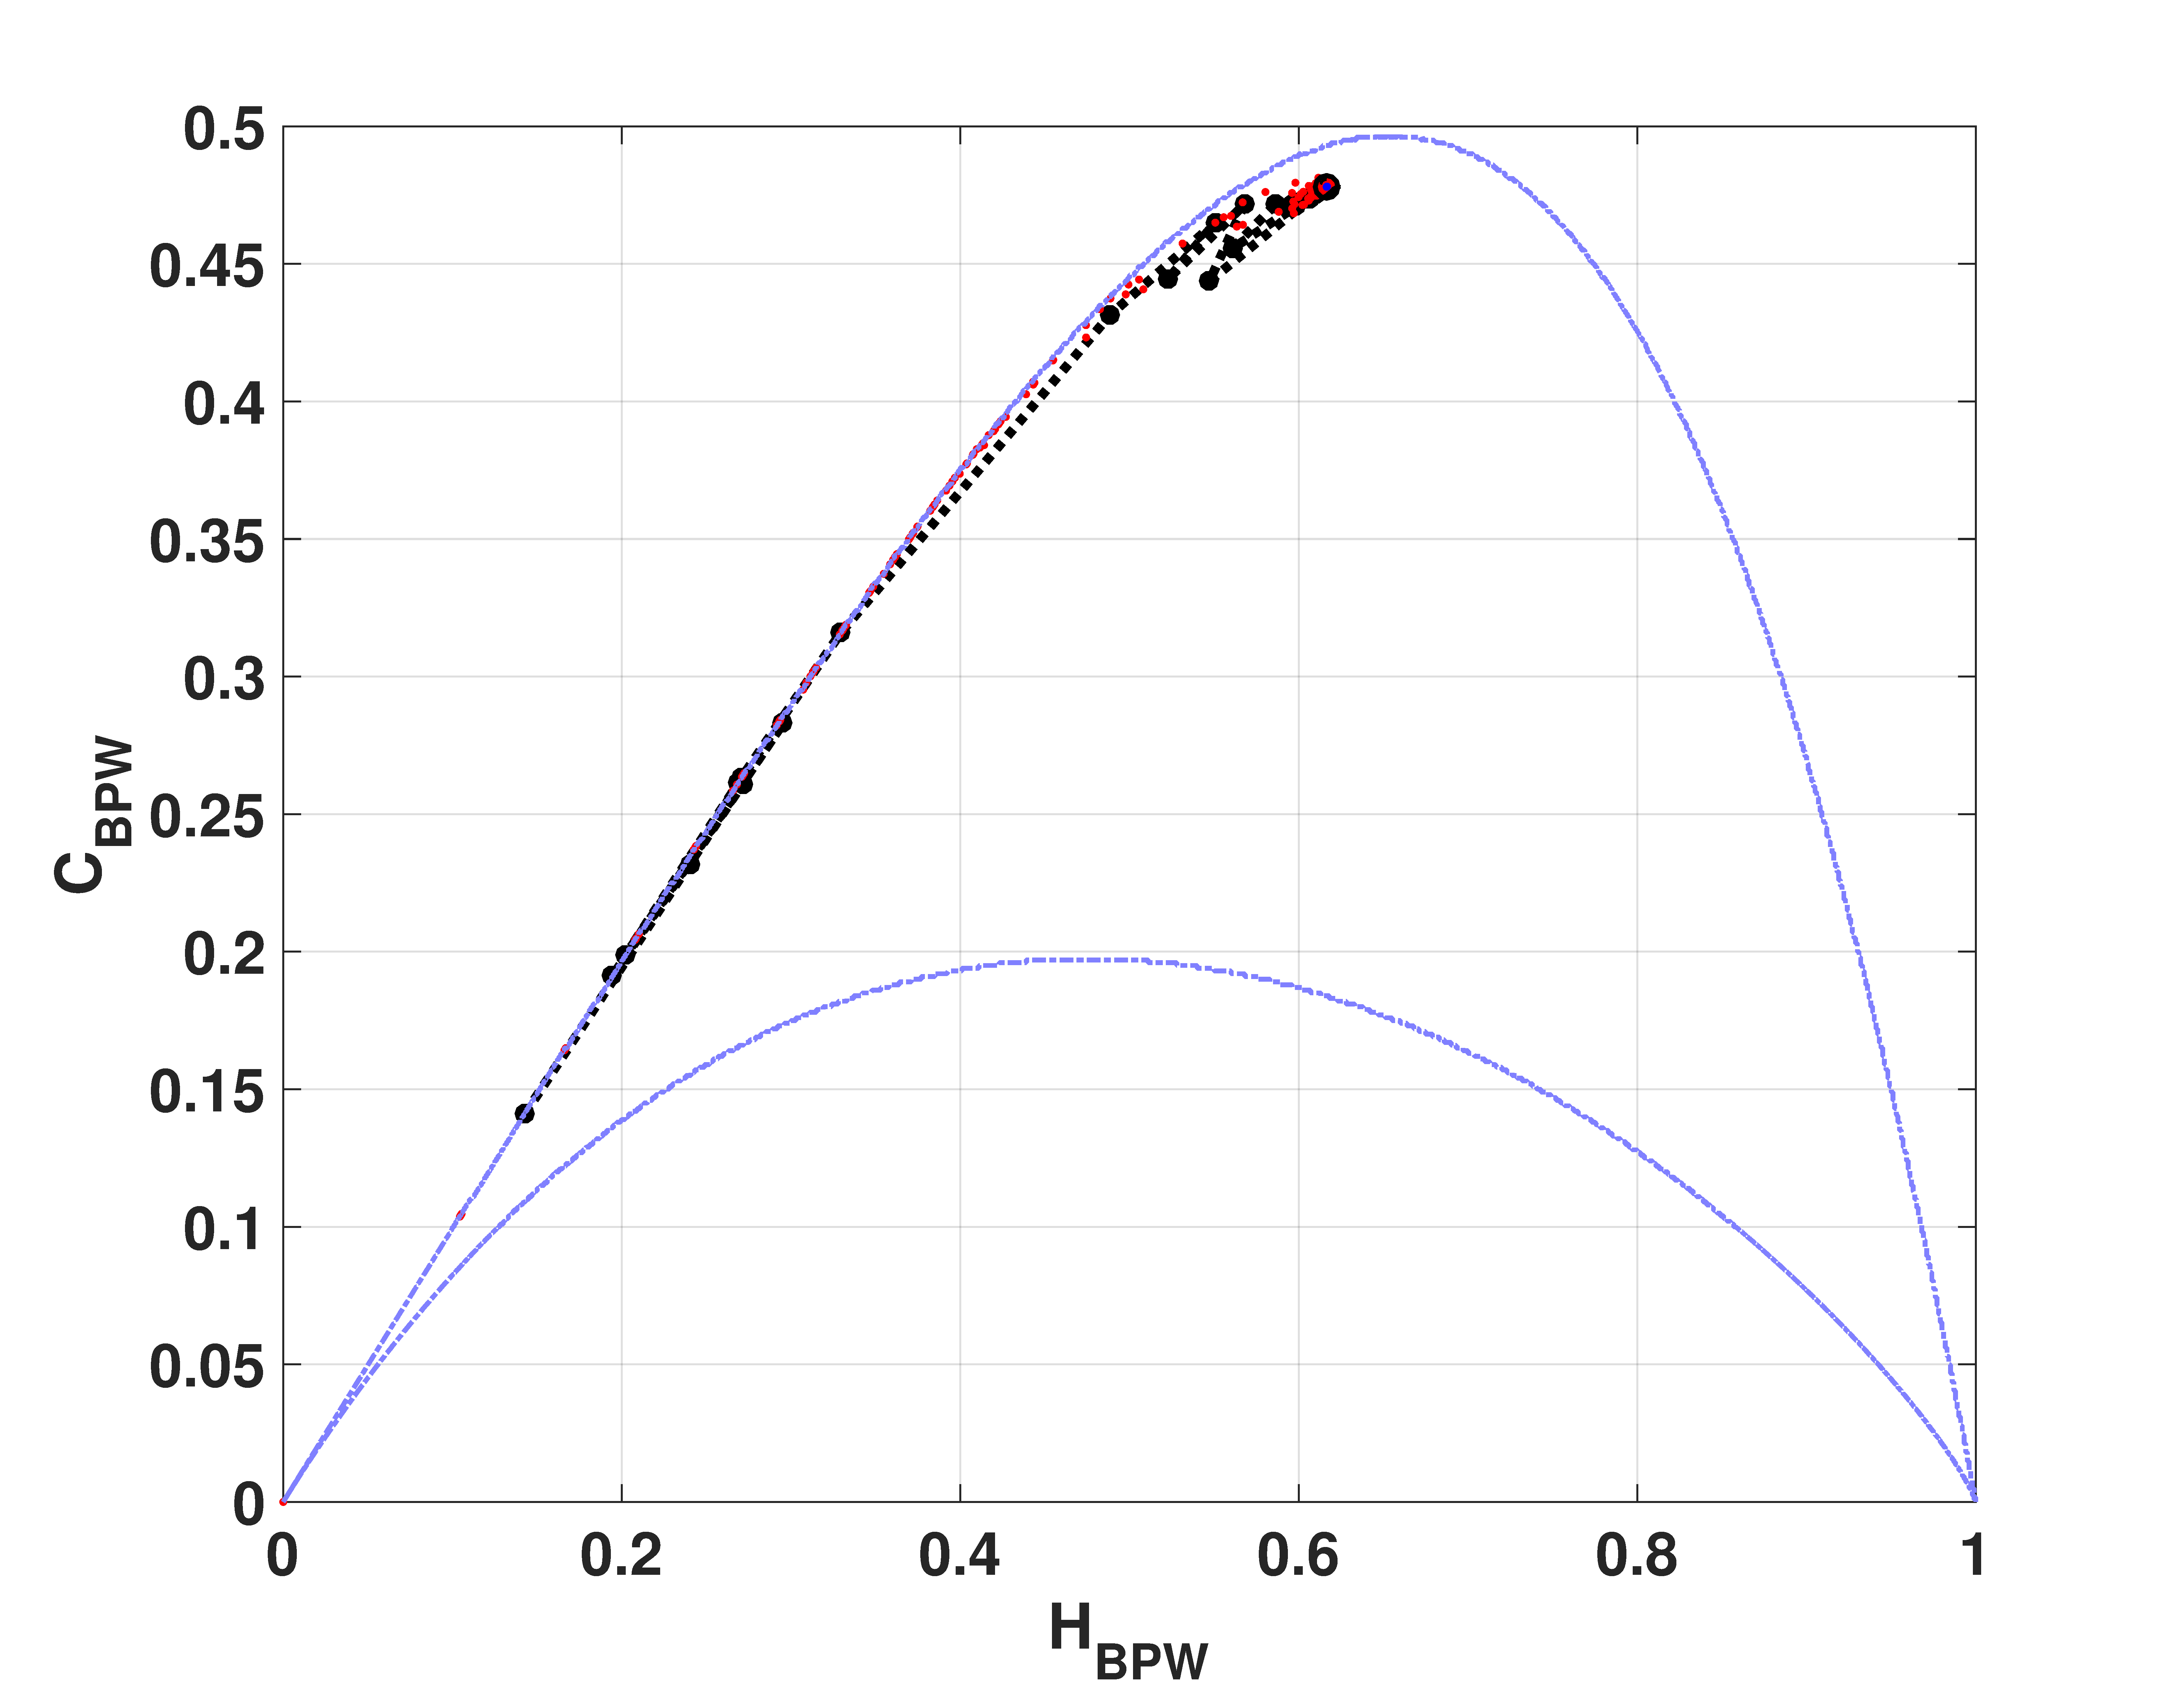
\includegraphics[width=.32\textwidth]{CbpwHbpw_Logistico}
	\caption{Statistical properties of the LOG map using binary representation: (a) $H_{hist}$ vs $P$ (b) $H_{BP}$ vs $P$ (c) $C_{BP}$ vs $P$ (d) Number of missing ordering patterns $MP$ vs $P$. In Figures (a) to (d) dashed line correspond to floating point numbers. (d) representation in the $H_{hist},H_{BP}$ plane in the the decimal numerical system.  The star represents the state for floating points numbers. (e) representation in the $H_{hist},H_{BP}$ plane. The star represents the state for floating point numbers; (f) representation in the $H_{BP},C_{BP}$ plane.  The star represents the state for floating points numbers. (f) representation in the $H_{BP},C_{BP}$ plane for binary numerical system.  The star represents the state for floating points numbers. } \label{fig:LOGbinario}
\end{figure}
